\documentclass[a4paper]{book}
\usepackage{makeidx}
\usepackage{natbib}
\usepackage{graphicx}
\usepackage{multicol}
\usepackage{float}
\usepackage{listings}
\usepackage{color}
\usepackage{ifthen}
\usepackage[table]{xcolor}
\usepackage{textcomp}
\usepackage{alltt}
\usepackage{ifpdf}
\ifpdf
\usepackage[pdftex,
            pagebackref=true,
            colorlinks=true,
            linkcolor=blue,
            unicode
           ]{hyperref}
\else
\usepackage[ps2pdf,
            pagebackref=true,
            colorlinks=true,
            linkcolor=blue,
            unicode
           ]{hyperref}
\usepackage{pspicture}
\fi
\usepackage[utf8]{inputenc}
\usepackage{mathptmx}
\usepackage[scaled=.90]{helvet}
\usepackage{courier}
\usepackage{sectsty}
\usepackage[titles]{tocloft}
\usepackage{doxygen}
\lstset{language=C++,inputencoding=utf8,basicstyle=\footnotesize,breaklines=true,breakatwhitespace=true,tabsize=8,numbers=left }
\makeindex
\setcounter{tocdepth}{3}
\renewcommand{\footrulewidth}{0.4pt}
\renewcommand{\familydefault}{\sfdefault}
\hfuzz=15pt
\setlength{\emergencystretch}{15pt}
\hbadness=750
\tolerance=750
\begin{document}
\hypersetup{pageanchor=false,citecolor=blue}
\begin{titlepage}
\vspace*{7cm}
\begin{center}
{\Large \-Anima \\[1ex]\large 0.\-9 }\\
\vspace*{1cm}
{\large \-Generated by Doxygen 1.7.6.1}\\
\vspace*{0.5cm}
{\small Wed Apr 25 2012 12:02:13}\\
\end{center}
\end{titlepage}
\clearemptydoublepage
\pagenumbering{roman}
\tableofcontents
\clearemptydoublepage
\pagenumbering{arabic}
\hypersetup{pageanchor=true,citecolor=blue}
\chapter{\-Class \-Index}
\section{\-Class \-Hierarchy}
\-This inheritance list is sorted roughly, but not completely, alphabetically\-:\begin{DoxyCompactList}
\item \contentsline{section}{\-Async\-Query}{\pageref{classAsyncQuery}}{}
\item \contentsline{section}{\-Async\-Query\-Result}{\pageref{structAsyncQueryResult}}{}
\item \contentsline{section}{\-Atomic\-Boolean}{\pageref{classAtomicBoolean}}{}
\item \contentsline{section}{\-Atomic\-Float}{\pageref{classAtomicFloat}}{}
\item \contentsline{section}{\-Atomic\-U\-Int}{\pageref{classAtomicUInt}}{}
\begin{DoxyCompactList}
\item \contentsline{section}{\-Atomic\-Counter}{\pageref{classAtomicCounter}}{}
\end{DoxyCompactList}
\item \contentsline{section}{\-Atomic\-U\-Long}{\pageref{classAtomicULong}}{}
\item \contentsline{section}{\-Boss\-Fight\-Control}{\pageref{classBossFightControl}}{}
\item \contentsline{section}{\-Callback\-Base}{\pageref{classCallbackBase}}{}
\begin{DoxyCompactList}
\item \contentsline{section}{\-Call\-Back\-Function\-P0}{\pageref{classCallBackFunctionP0}}{}
\item \contentsline{section}{\-Call\-Back\-Function\-P1$<$ \-P1 $>$}{\pageref{classCallBackFunctionP1}}{}
\item \contentsline{section}{\-Call\-Back\-Function\-P2$<$ \-P1, \-P2 $>$}{\pageref{classCallBackFunctionP2}}{}
\item \contentsline{section}{\-Call\-Back\-Function\-P3$<$ \-P1, \-P2, \-P3 $>$}{\pageref{classCallBackFunctionP3}}{}
\item \contentsline{section}{\-Call\-Back\-Function\-P4$<$ \-P1, \-P2, \-P3, \-P4 $>$}{\pageref{classCallBackFunctionP4}}{}
\item \contentsline{section}{\-Callback\-P0$<$ \-Class $>$}{\pageref{classCallbackP0}}{}
\item \contentsline{section}{\-Callback\-P1$<$ \-Class, \-P1 $>$}{\pageref{classCallbackP1}}{}
\item \contentsline{section}{\-Callback\-P2$<$ \-Class, \-P1, \-P2 $>$}{\pageref{classCallbackP2}}{}
\item \contentsline{section}{\-Callback\-P3$<$ \-Class, \-P1, \-P2, \-P3 $>$}{\pageref{classCallbackP3}}{}
\item \contentsline{section}{\-Callback\-P4$<$ \-Class, \-P1, \-P2, \-P3, \-P4 $>$}{\pageref{classCallbackP4}}{}
\end{DoxyCompactList}
\item \contentsline{section}{\-Callback\-F\-P}{\pageref{classCallbackFP}}{}
\item \contentsline{section}{\-C\-Int64}{\pageref{structCInt64}}{}
\item \contentsline{section}{\-Database\-Connection}{\pageref{structDatabaseConnection}}{}
\begin{DoxyCompactList}
\item \contentsline{section}{\-My\-S\-Q\-L\-Database\-Connection}{\pageref{structMySQLDatabaseConnection}}{}
\end{DoxyCompactList}
\item \contentsline{section}{\-Dict\-Give}{\pageref{structDictGive}}{}
\item \contentsline{section}{\-Dict\-J\-S\-O\-N\-Generator}{\pageref{classDictJSONGenerator}}{}
\item \contentsline{section}{\-Dict\-Object}{\pageref{classDictObject}}{}
\item \contentsline{section}{\-Dict\-Pack}{\pageref{structDictPack}}{}
\item \contentsline{section}{\-Error\-Exeption}{\pageref{classErrorExeption}}{}
\item \contentsline{section}{\-Ext\-Connection}{\pageref{structExtConnection}}{}
\item \contentsline{section}{\-Ext\-Server\-Connection}{\pageref{classExtServerConnection}}{}
\item \contentsline{section}{\-Fast\-Mutex}{\pageref{classFastMutex}}{}
\item \contentsline{section}{\-Fast\-R\-W\-Mutex}{\pageref{classFastRWMutex}}{}
\item \contentsline{section}{\-Field}{\pageref{classField}}{}
\item \contentsline{section}{\-F\-Queue$<$ \-T $>$}{\pageref{classFQueue}}{}
\item \contentsline{section}{\-I\-G\-\_\-2\-Int32}{\pageref{structIG__2Int32}}{}
\item \contentsline{section}{\-I\-G\-\_\-\-Int32}{\pageref{structIG__Int32}}{}
\item \contentsline{section}{\-I\-G\-\_\-\-J\-O\-I\-N}{\pageref{structIG__JOIN}}{}
\item \contentsline{section}{\-Instance}{\pageref{classInstance}}{}
\begin{DoxyCompactList}
\item \contentsline{section}{\-Ext\-Socket\-Instance}{\pageref{classExtSocketInstance}}{}
\item \contentsline{section}{\-Main\-Instance}{\pageref{classMainInstance}}{}
\end{DoxyCompactList}
\item \contentsline{section}{\-J\-S\-O\-N}{\pageref{classJSON}}{}
\item \contentsline{section}{\-J\-S\-O\-N\-Value}{\pageref{classJSONValue}}{}
\item \contentsline{section}{\-Kick}{\pageref{structKick}}{}
\item \contentsline{section}{location}{\pageref{classlocation}}{}
\item \contentsline{section}{\-Mutex}{\pageref{classMutex}}{}
\item \contentsline{section}{\-Object}{\pageref{classObject}}{}
\item \contentsline{section}{\-Object\-List}{\pageref{classObjectList}}{}
\item \contentsline{section}{\-O\-G\-\_\-\-E\-R\-R\-O\-R}{\pageref{structOG__ERROR}}{}
\item \contentsline{section}{\-O\-G\-\_\-\-U\-S\-E\-R\-\_\-\-J\-S\-O\-N}{\pageref{structOG__USER__JSON}}{}
\item \contentsline{section}{\-Packet}{\pageref{structPacket}}{}
\item \contentsline{section}{\-Packet\-Handler$<$ \-T $>$}{\pageref{classPacketHandler}}{}
\item \contentsline{section}{\-Periodic\-Thread}{\pageref{structPeriodicThread}}{}
\item \contentsline{section}{\-Query\-Buffer}{\pageref{classQueryBuffer}}{}
\item \contentsline{section}{\-Query\-Result}{\pageref{classQueryResult}}{}
\begin{DoxyCompactList}
\item \contentsline{section}{\-My\-S\-Q\-L\-Query\-Result}{\pageref{classMySQLQueryResult}}{}
\end{DoxyCompactList}
\item \contentsline{section}{\-Rating\-Manager}{\pageref{classRatingManager}}{}
\item \contentsline{section}{\-Reference\-Counter}{\pageref{classReferenceCounter}}{}
\item \contentsline{section}{\-Singleton$<$ type $>$}{\pageref{classSingleton}}{}
\item \contentsline{section}{\-Singleton$<$ \-Config $>$}{\pageref{classSingleton}}{}
\begin{DoxyCompactList}
\item \contentsline{section}{\-Config}{\pageref{classConfig}}{}
\end{DoxyCompactList}
\item \contentsline{section}{\-Singleton$<$ \-Database\-Manager $>$}{\pageref{classSingleton}}{}
\begin{DoxyCompactList}
\item \contentsline{section}{\-Database\-Manager}{\pageref{classDatabaseManager}}{}
\end{DoxyCompactList}
\item \contentsline{section}{\-Singleton$<$ \-Dict\-Manager $>$}{\pageref{classSingleton}}{}
\begin{DoxyCompactList}
\item \contentsline{section}{\-Dict\-Manager}{\pageref{classDictManager}}{}
\end{DoxyCompactList}
\item \contentsline{section}{\-Singleton$<$ \-Ext\-Server\-Manager $>$}{\pageref{classSingleton}}{}
\begin{DoxyCompactList}
\item \contentsline{section}{\-Ext\-Server\-Manager}{\pageref{classExtServerManager}}{}
\end{DoxyCompactList}
\item \contentsline{section}{\-Singleton$<$ \-Net\-Core $>$}{\pageref{classSingleton}}{}
\begin{DoxyCompactList}
\item \contentsline{section}{\-Net\-Core}{\pageref{classNetCore}}{}
\end{DoxyCompactList}
\item \contentsline{section}{\-Singleton$<$ \-Periodic\-Thread\-Caller $>$}{\pageref{classSingleton}}{}
\begin{DoxyCompactList}
\item \contentsline{section}{\-Periodic\-Thread\-Caller}{\pageref{classPeriodicThreadCaller}}{}
\end{DoxyCompactList}
\item \contentsline{section}{\-Singleton$<$ \-Random $>$}{\pageref{classSingleton}}{}
\begin{DoxyCompactList}
\item \contentsline{section}{\-Random}{\pageref{classRandom}}{}
\end{DoxyCompactList}
\item \contentsline{section}{\-Singleton$<$ \-Server $>$}{\pageref{classSingleton}}{}
\begin{DoxyCompactList}
\item \contentsline{section}{\-Server}{\pageref{classServer}}{}
\begin{DoxyCompactList}
\item \contentsline{section}{\-Game\-Server}{\pageref{classGameServer}}{}
\end{DoxyCompactList}
\end{DoxyCompactList}
\item \contentsline{section}{\-Singleton$<$ \-Storage $>$}{\pageref{classSingleton}}{}
\begin{DoxyCompactList}
\item \contentsline{section}{\-Storage}{\pageref{classStorage}}{}
\end{DoxyCompactList}
\item \contentsline{section}{\-Singleton$<$ \-Thread\-Core $>$}{\pageref{classSingleton}}{}
\begin{DoxyCompactList}
\item \contentsline{section}{\-Thread\-Core}{\pageref{classThreadCore}}{}
\end{DoxyCompactList}
\item \contentsline{section}{\-Singleton$<$ \-Version\-Control $>$}{\pageref{classSingleton}}{}
\begin{DoxyCompactList}
\item \contentsline{section}{\-Version\-Control}{\pageref{classVersionControl}}{}
\end{DoxyCompactList}
\item \contentsline{section}{\-Smart\-Ptr$<$ \-T $>$}{\pageref{classSmartPtr}}{}
\item \contentsline{section}{\-Social\-Net\-Desc}{\pageref{structSocialNetDesc}}{}
\item \contentsline{section}{\-Socket\-Base}{\pageref{classSocketBase}}{}
\begin{DoxyCompactList}
\item \contentsline{section}{\-Socket\-Operations}{\pageref{classSocketOperations}}{}
\begin{DoxyCompactList}
\item \contentsline{section}{\-Socket}{\pageref{classSocket}}{}
\begin{DoxyCompactList}
\item \contentsline{section}{\-Listen\-Socket}{\pageref{classListenSocket}}{}
\begin{DoxyCompactList}
\item \contentsline{section}{\-Ext\-Socket}{\pageref{classExtSocket}}{}
\item \contentsline{section}{\-Game\-Socket}{\pageref{classGameSocket}}{}
\item \contentsline{section}{\-Login\-Socket}{\pageref{classLoginSocket}}{}
\end{DoxyCompactList}
\end{DoxyCompactList}
\end{DoxyCompactList}
\end{DoxyCompactList}
\item \contentsline{section}{\-S\-Q\-L\-Callback\-Base}{\pageref{classSQLCallbackBase}}{}
\begin{DoxyCompactList}
\item \contentsline{section}{\-S\-Q\-L\-Class\-Callback\-P0$<$ \-T $>$}{\pageref{classSQLClassCallbackP0}}{}
\item \contentsline{section}{\-S\-Q\-L\-Class\-Callback\-P1$<$ \-T, \-P1 $>$}{\pageref{classSQLClassCallbackP1}}{}
\item \contentsline{section}{\-S\-Q\-L\-Class\-Callback\-P2$<$ \-T, \-P1, \-P2 $>$}{\pageref{classSQLClassCallbackP2}}{}
\item \contentsline{section}{\-S\-Q\-L\-Class\-Callback\-P3$<$ \-T, \-P1, \-P2, \-P3 $>$}{\pageref{classSQLClassCallbackP3}}{}
\item \contentsline{section}{\-S\-Q\-L\-Class\-Callback\-P4$<$ \-T, \-P1, \-P2, \-P3, \-P4 $>$}{\pageref{classSQLClassCallbackP4}}{}
\item \contentsline{section}{\-S\-Q\-L\-Function\-Callback\-P0}{\pageref{classSQLFunctionCallbackP0}}{}
\item \contentsline{section}{\-S\-Q\-L\-Function\-Callback\-P1$<$ \-T1 $>$}{\pageref{classSQLFunctionCallbackP1}}{}
\end{DoxyCompactList}
\item \contentsline{section}{\-Thread}{\pageref{classThread}}{}
\begin{DoxyCompactList}
\item \contentsline{section}{\-Database}{\pageref{classDatabase}}{}
\begin{DoxyCompactList}
\item \contentsline{section}{\-My\-S\-Q\-L\-Database}{\pageref{classMySQLDatabase}}{}
\end{DoxyCompactList}
\item \contentsline{section}{\-Debug\-Update}{\pageref{classDebugUpdate}}{}
\item \contentsline{section}{\-Ext\-Socket\-Thread}{\pageref{classExtSocketThread}}{}
\item \contentsline{section}{\-Game\-Socket\-Thread}{\pageref{classGameSocketThread}}{}
\item \contentsline{section}{\-Login\-Socket\-Thread}{\pageref{classLoginSocketThread}}{}
\item \contentsline{section}{\-Net\-Core\-Worker\-Thread}{\pageref{classNetCoreWorkerThread}}{}
\item \contentsline{section}{\-Periodic\-Thread\-Caller}{\pageref{classPeriodicThreadCaller}}{}
\item \contentsline{section}{\-Query\-Thread}{\pageref{classQueryThread}}{}
\item \contentsline{section}{\-Storage\-Thread}{\pageref{classStorageThread}}{}
\item \contentsline{section}{\-Storage\-Timer}{\pageref{classStorageTimer}}{}
\end{DoxyCompactList}
\item \contentsline{section}{\-Thread\-Controller}{\pageref{classThreadController}}{}
\item \contentsline{section}{\-User}{\pageref{classUser}}{}
\item \contentsline{section}{\-User\-Interface}{\pageref{classUserInterface}}{}
\begin{DoxyCompactList}
\item \contentsline{section}{\-User\-Ext}{\pageref{classUserExt}}{}
\end{DoxyCompactList}
\item \contentsline{section}{\-Value}{\pageref{classValue}}{}
\item \contentsline{section}{\-V\-C\-Base}{\pageref{classVCBase}}{}
\begin{DoxyCompactList}
\item \contentsline{section}{\-Git\-V\-C}{\pageref{classGitVC}}{}
\end{DoxyCompactList}
\end{DoxyCompactList}

\chapter{\-Class \-Index}
\section{Class List}
Here are the classes, structs, unions and interfaces with brief descriptions:\begin{DoxyCompactList}
\item\contentsline{section}{\hyperlink{classAtomicBoolean}{AtomicBoolean} }{\pageref{classAtomicBoolean}}{}
\item\contentsline{section}{\hyperlink{classAtomicCounter}{AtomicCounter} }{\pageref{classAtomicCounter}}{}
\item\contentsline{section}{\hyperlink{classAtomicFloat}{AtomicFloat} }{\pageref{classAtomicFloat}}{}
\item\contentsline{section}{\hyperlink{classAtomicUInt}{AtomicUInt} }{\pageref{classAtomicUInt}}{}
\item\contentsline{section}{\hyperlink{classAtomicULong}{AtomicULong} }{\pageref{classAtomicULong}}{}
\item\contentsline{section}{\hyperlink{classConfig}{Config} (Server configuration data store )}{\pageref{classConfig}}{}
\item\contentsline{section}{\hyperlink{classFastMutex}{FastMutex} (\hyperlink{classMutex}{Mutex} for short locks )}{\pageref{classFastMutex}}{}
\item\contentsline{section}{\hyperlink{classFastRWMutex}{FastRWMutex} (\hyperlink{classMutex}{Mutex} for RW short locks )}{\pageref{classFastRWMutex}}{}
\item\contentsline{section}{\hyperlink{classFQueue}{FQueue$<$ T $>$} }{\pageref{classFQueue}}{}
\item\contentsline{section}{\hyperlink{classJSON}{JSON} }{\pageref{classJSON}}{}
\item\contentsline{section}{\hyperlink{classJSONValue}{JSONValue} }{\pageref{classJSONValue}}{}
\item\contentsline{section}{\hyperlink{classListenSocket}{ListenSocket$<$ SocketClass $>$} }{\pageref{classListenSocket}}{}
\item\contentsline{section}{\hyperlink{classListenSocketBase}{ListenSocketBase} }{\pageref{classListenSocketBase}}{}
\item\contentsline{section}{\hyperlink{classLoginServer}{LoginServer} }{\pageref{classLoginServer}}{}
\item\contentsline{section}{\hyperlink{classLSHandlerSocket}{LSHandlerSocket} }{\pageref{classLSHandlerSocket}}{}
\item\contentsline{section}{\hyperlink{classLSWorkerThread}{LSWorkerThread} }{\pageref{classLSWorkerThread}}{}
\item\contentsline{section}{\hyperlink{classMutex}{Mutex} }{\pageref{classMutex}}{}
\item\contentsline{section}{\hyperlink{classNetCore}{NetCore} }{\pageref{classNetCore}}{}
\item\contentsline{section}{\hyperlink{classNetCoreWorkerThread}{NetCoreWorkerThread} }{\pageref{classNetCoreWorkerThread}}{}
\item\contentsline{section}{\hyperlink{structPacket}{Packet} }{\pageref{structPacket}}{}
\item\contentsline{section}{\hyperlink{structPeriodicThread}{PeriodicThread} }{\pageref{structPeriodicThread}}{}
\item\contentsline{section}{\hyperlink{classPeriodicThreadCaller}{PeriodicThreadCaller} }{\pageref{classPeriodicThreadCaller}}{}
\item\contentsline{section}{\hyperlink{classSingleton}{Singleton$<$ type $>$} }{\pageref{classSingleton}}{}
\item\contentsline{section}{\hyperlink{classSocket}{Socket} }{\pageref{classSocket}}{}
\item\contentsline{section}{\hyperlink{classSocketBase}{SocketBase} }{\pageref{classSocketBase}}{}
\item\contentsline{section}{\hyperlink{classSocketOperations}{SocketOperations} }{\pageref{classSocketOperations}}{}
\item\contentsline{section}{\hyperlink{classThread}{Thread} }{\pageref{classThread}}{}
\item\contentsline{section}{\hyperlink{classThreadController}{ThreadController} }{\pageref{classThreadController}}{}
\item\contentsline{section}{\hyperlink{classThreadCore}{ThreadCore} }{\pageref{classThreadCore}}{}
\end{DoxyCompactList}

\chapter{\-Class \-Documentation}
\input{classAsyncQuery}
\input{structAsyncQueryResult}
\hypertarget{classAtomicBoolean}{\section{\-Atomic\-Boolean \-Class \-Reference}
\label{classAtomicBoolean}\index{\-Atomic\-Boolean@{\-Atomic\-Boolean}}
}
\subsection*{\-Public \-Member \-Functions}
\begin{DoxyCompactItemize}
\item 
\hypertarget{classAtomicBoolean_a562a704c03897cbaf8f95b73d1e63df0}{{\bfseries \-Atomic\-Boolean} (bool val)}\label{classAtomicBoolean_a562a704c03897cbaf8f95b73d1e63df0}

\item 
\hypertarget{classAtomicBoolean_a7f1816ac1fb9d992f830bcf64a56a5ab}{bool {\bfseries set\-Val} (bool val)}\label{classAtomicBoolean_a7f1816ac1fb9d992f830bcf64a56a5ab}

\item 
\hypertarget{classAtomicBoolean_a564480e3423763ec212471429d9bd659}{bool {\bfseries get\-Val} ()}\label{classAtomicBoolean_a564480e3423763ec212471429d9bd659}

\end{DoxyCompactItemize}


\-The documentation for this class was generated from the following files\-:\begin{DoxyCompactItemize}
\item 
/home/nonametr/projects/voodoo/server/shared/mt/thread.\-h\item 
/home/nonametr/projects/voodoo/server/shared/mt/thread.\-cpp\end{DoxyCompactItemize}

\hypertarget{classAtomicCounter}{\section{\-Atomic\-Counter \-Class \-Reference}
\label{classAtomicCounter}\index{\-Atomic\-Counter@{\-Atomic\-Counter}}
}
\-Inheritance diagram for \-Atomic\-Counter\-:\begin{figure}[H]
\begin{center}
\leavevmode
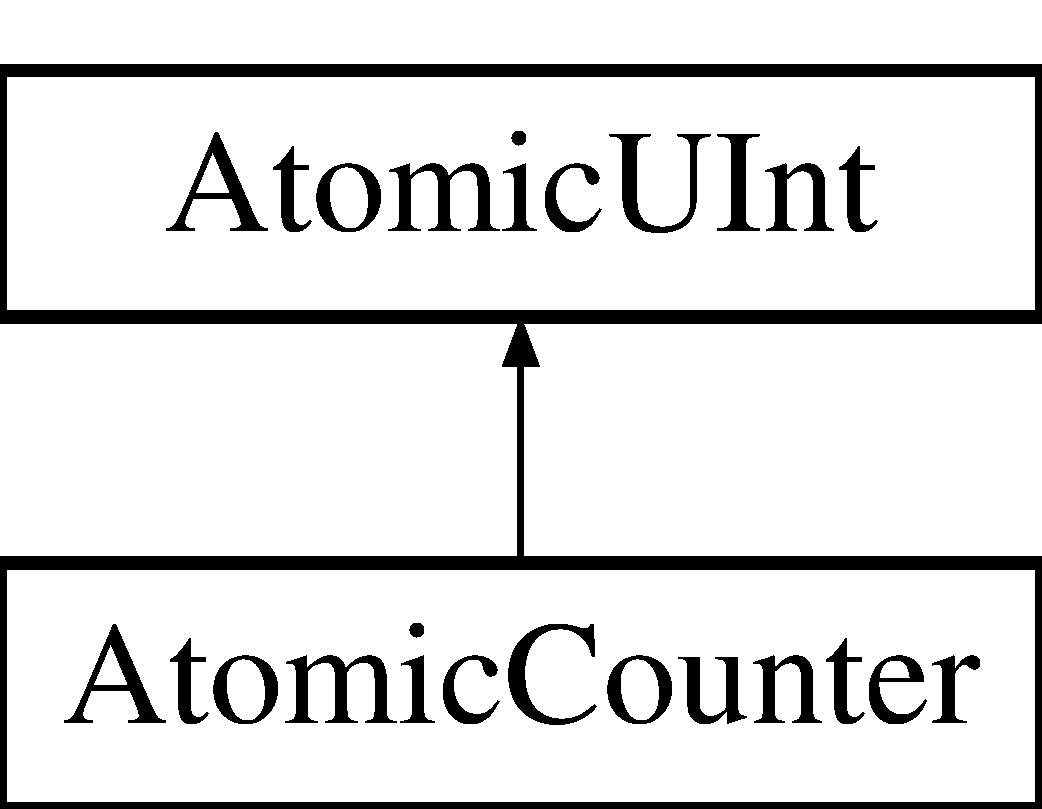
\includegraphics[height=2.000000cm]{classAtomicCounter}
\end{center}
\end{figure}
\subsection*{\-Public \-Member \-Functions}
\begin{DoxyCompactItemize}
\item 
\hypertarget{classAtomicCounter_a7ac0a9d0ea94c1d44085643b013e6691}{{\bfseries \-Atomic\-Counter} (unsigned int \-Initial\-Value)}\label{classAtomicCounter_a7ac0a9d0ea94c1d44085643b013e6691}

\item 
\hypertarget{classAtomicCounter_a67e47216267c256c7236b2612969a2b1}{unsigned int {\bfseries operator++} ()}\label{classAtomicCounter_a67e47216267c256c7236b2612969a2b1}

\item 
\hypertarget{classAtomicCounter_a464033cba228a18de3b93344b131a638}{unsigned int {\bfseries operator-\/-\/} ()}\label{classAtomicCounter_a464033cba228a18de3b93344b131a638}

\end{DoxyCompactItemize}


\-The documentation for this class was generated from the following files\-:\begin{DoxyCompactItemize}
\item 
/home/nonametr/projects/voodoo/server/shared/mt/thread.\-h\item 
/home/nonametr/projects/voodoo/server/shared/mt/thread.\-cpp\end{DoxyCompactItemize}

\hypertarget{classAtomicFloat}{\section{\-Atomic\-Float \-Class \-Reference}
\label{classAtomicFloat}\index{\-Atomic\-Float@{\-Atomic\-Float}}
}
\subsection*{\-Public \-Member \-Functions}
\begin{DoxyCompactItemize}
\item 
\hypertarget{classAtomicFloat_a3b18907aa5d736361d0711bbb53b23b0}{{\bfseries \-Atomic\-Float} (float \-Initial\-Value)}\label{classAtomicFloat_a3b18907aa5d736361d0711bbb53b23b0}

\item 
\hypertarget{classAtomicFloat_a4e59fd811f0cf118e5be5c278374a060}{float {\bfseries set\-Val} (float \-New\-Value)}\label{classAtomicFloat_a4e59fd811f0cf118e5be5c278374a060}

\item 
\hypertarget{classAtomicFloat_accd3d0c651d3ee96078ecff6416ef8e1}{float {\bfseries get\-Val} ()}\label{classAtomicFloat_accd3d0c651d3ee96078ecff6416ef8e1}

\end{DoxyCompactItemize}


\-The documentation for this class was generated from the following files\-:\begin{DoxyCompactItemize}
\item 
/home/nonametr/projects/voodoo/server/shared/mt/thread.\-h\item 
/home/nonametr/projects/voodoo/server/shared/mt/thread.\-cpp\end{DoxyCompactItemize}

\hypertarget{classAtomicUInt}{\section{\-Atomic\-U\-Int \-Class \-Reference}
\label{classAtomicUInt}\index{\-Atomic\-U\-Int@{\-Atomic\-U\-Int}}
}
\-Inheritance diagram for \-Atomic\-U\-Int\-:\begin{figure}[H]
\begin{center}
\leavevmode
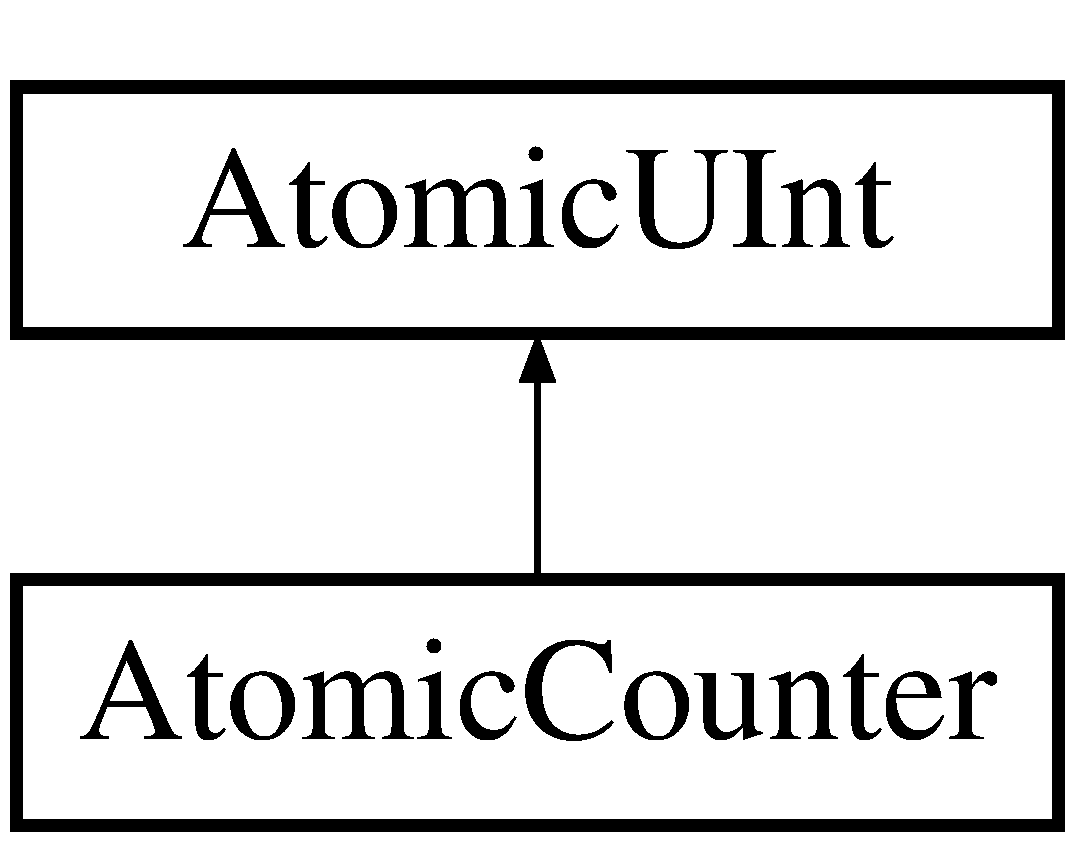
\includegraphics[height=2.000000cm]{classAtomicUInt}
\end{center}
\end{figure}
\subsection*{\-Public \-Member \-Functions}
\begin{DoxyCompactItemize}
\item 
\hypertarget{classAtomicUInt_a65bd3ad3493bd2f2797db73aacce9882}{{\bfseries \-Atomic\-U\-Int} (unsigned int \-Initial\-Value)}\label{classAtomicUInt_a65bd3ad3493bd2f2797db73aacce9882}

\item 
\hypertarget{classAtomicUInt_ae82f87c778d1fd9e67fb1f775f1dd57c}{unsigned int {\bfseries add\-Val} (unsigned int \-Add\-Value)}\label{classAtomicUInt_ae82f87c778d1fd9e67fb1f775f1dd57c}

\item 
\hypertarget{classAtomicUInt_a18db8edb0b877d5a8318c14396821b17}{unsigned int {\bfseries sub\-Val} (unsigned int \-Sub\-Value)}\label{classAtomicUInt_a18db8edb0b877d5a8318c14396821b17}

\item 
\hypertarget{classAtomicUInt_a6c87f086b485602617626075cd93f195}{unsigned int {\bfseries set\-Val} (unsigned int \-New\-Value)}\label{classAtomicUInt_a6c87f086b485602617626075cd93f195}

\item 
\hypertarget{classAtomicUInt_ab63ca35550efe69346e79b52c4670125}{unsigned int {\bfseries get\-Val} ()}\label{classAtomicUInt_ab63ca35550efe69346e79b52c4670125}

\end{DoxyCompactItemize}
\subsection*{\-Protected \-Attributes}
\begin{DoxyCompactItemize}
\item 
\hypertarget{classAtomicUInt_aba7c56a82dffafaa622adfe4ec09d2ca}{volatile unsigned int {\bfseries \-Value}}\label{classAtomicUInt_aba7c56a82dffafaa622adfe4ec09d2ca}

\end{DoxyCompactItemize}


\-The documentation for this class was generated from the following file\-:\begin{DoxyCompactItemize}
\item 
/home/nonametr/projects/voodoo/server/shared/mt/thread.\-h\end{DoxyCompactItemize}

\hypertarget{classAtomicULong}{
\section{AtomicULong Class Reference}
\label{classAtomicULong}\index{AtomicULong@{AtomicULong}}
}
\subsection*{Public Member Functions}
\begin{DoxyCompactItemize}
\item 
\hypertarget{classAtomicULong_a3a096a93ad40cda8bee202c76e2681e6}{
{\bfseries AtomicULong} (unsigned long InitialValue)}
\label{classAtomicULong_a3a096a93ad40cda8bee202c76e2681e6}

\item 
\hypertarget{classAtomicULong_a47dc532a4af8bfc3ab1c8e582b75c6cf}{
unsigned int {\bfseries SetVal} (unsigned long NewValue)}
\label{classAtomicULong_a47dc532a4af8bfc3ab1c8e582b75c6cf}

\item 
\hypertarget{classAtomicULong_a081cc984d0cb34a4eaa067f511db3c5c}{
unsigned int {\bfseries AddVal} (unsigned long AddValue)}
\label{classAtomicULong_a081cc984d0cb34a4eaa067f511db3c5c}

\item 
\hypertarget{classAtomicULong_a6b12a59005990ca71bcf8356c7131d09}{
unsigned int {\bfseries GetVal} ()}
\label{classAtomicULong_a6b12a59005990ca71bcf8356c7131d09}

\end{DoxyCompactItemize}
\subsection*{Protected Attributes}
\begin{DoxyCompactItemize}
\item 
\hypertarget{classAtomicULong_a65f08ef36d8f8160866d1c8a15dd47af}{
volatile unsigned long {\bfseries Value}}
\label{classAtomicULong_a65f08ef36d8f8160866d1c8a15dd47af}

\end{DoxyCompactItemize}


The documentation for this class was generated from the following files:\begin{DoxyCompactItemize}
\item 
/home/nonametr/projects/anima/shared/thread.h\item 
/home/nonametr/projects/anima/shared/thread.cpp\end{DoxyCompactItemize}

\input{classBossFightControl}
\input{classCallbackBase}
\input{classCallbackFP}
\input{classCallBackFunctionP0}
\input{classCallBackFunctionP1}
\input{classCallBackFunctionP2}
\input{classCallBackFunctionP3}
\input{classCallBackFunctionP4}
\input{classCallbackP0}
\input{classCallbackP1}
\input{classCallbackP2}
\input{classCallbackP3}
\input{classCallbackP4}
\input{structCInt64}
\hypertarget{classConfig}{\section{\-Config \-Class \-Reference}
\label{classConfig}\index{\-Config@{\-Config}}
}


server configuration data store  




{\ttfamily \#include $<$config.\-h$>$}

\-Inheritance diagram for \-Config\-:\begin{figure}[H]
\begin{center}
\leavevmode
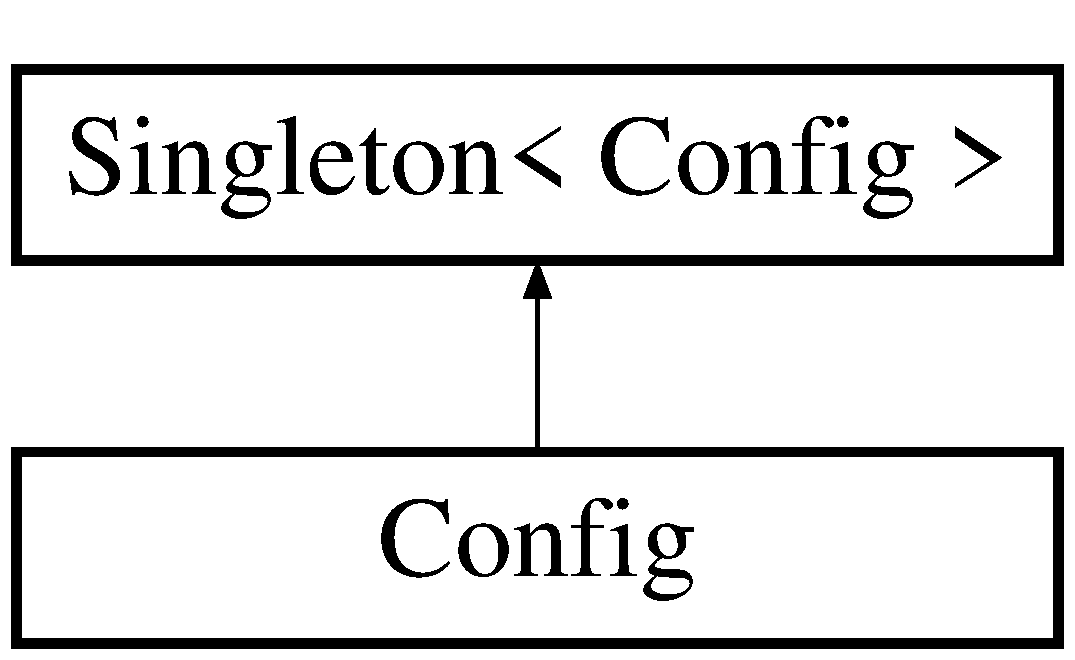
\includegraphics[height=2.000000cm]{classConfig}
\end{center}
\end{figure}
\subsection*{\-Public \-Types}
\begin{DoxyCompactItemize}
\item 
enum \hyperlink{classConfig_a6d78e4d65fd44d149ad6facce11bc11e}{\-C\-O\-N\-F\-I\-G\-\_\-\-P\-A\-R\-A\-M\-S\-\_\-\-S\-T\-R} \{ \*
\hyperlink{classConfig_a6d78e4d65fd44d149ad6facce11bc11eadb86d6ef5692400d4a3c0a2fe54dba3d}{\-S\-S\-D\-\_\-\-I\-P}, 
{\bfseries \-S\-S\-D\-\_\-\-N\-A\-M\-E}, 
{\bfseries \-S\-S\-D\-\_\-\-U\-S\-E\-R}, 
{\bfseries \-S\-S\-D\-\_\-\-P\-A\-S\-S\-W\-O\-R\-D}, 
\*
{\bfseries \-S\-S\-D\-\_\-\-C\-H\-A\-R\-S\-E\-T}, 
{\bfseries \-S\-I\-Z\-E\-\_\-\-S\-T\-R}
 \}
\begin{DoxyCompactList}\small\item\em all string params of server configuration discribed in this enum \end{DoxyCompactList}\item 
enum \hyperlink{classConfig_a0f80a094ada73f8574e85b160a5e47b7}{\-C\-O\-N\-F\-I\-G\-\_\-\-P\-A\-R\-A\-M\-S\-\_\-\-I\-N\-T} \{ \hyperlink{classConfig_a0f80a094ada73f8574e85b160a5e47b7adcfee10d7cec219fc657459ee83d642f}{\-S\-S\-D\-\_\-\-P\-O\-R\-T}, 
{\bfseries \-S\-I\-Z\-E\-\_\-\-I\-N\-T}
 \}
\begin{DoxyCompactList}\small\item\em all int params of server configuration discribed in this enum \end{DoxyCompactList}\end{DoxyCompactItemize}
\subsection*{\-Public \-Member \-Functions}
\begin{DoxyCompactItemize}
\item 
\hypertarget{classConfig_abd0c571c116924871e30444b192b792a}{\hyperlink{classConfig_abd0c571c116924871e30444b192b792a}{\-Config} ()}\label{classConfig_abd0c571c116924871e30444b192b792a}

\begin{DoxyCompactList}\small\item\em constructor performs loading all configurations params \end{DoxyCompactList}\item 
void \hyperlink{classConfig_a0a2ae073a94b6d495a6113e01a0563db}{load\-From\-File} (const char $\ast$cfg\-\_\-file)
\begin{DoxyCompactList}\small\item\em performs loading base configuration data from config file \end{DoxyCompactList}\item 
void \hyperlink{classConfig_a182d6c22c9a9e09b7a38b0339bc742b1}{load\-From\-D\-B} ()
\begin{DoxyCompactList}\small\item\em performs loading configuration data from database \end{DoxyCompactList}\item 
\hypertarget{classConfig_adb59977d3f13d7a1223e6c7523240c7b}{const int \& {\bfseries get\-Param} (\hyperlink{classConfig_a0f80a094ada73f8574e85b160a5e47b7}{\-C\-O\-N\-F\-I\-G\-\_\-\-P\-A\-R\-A\-M\-S\-\_\-\-I\-N\-T} int\-\_\-param)}\label{classConfig_adb59977d3f13d7a1223e6c7523240c7b}

\item 
\hypertarget{classConfig_a8e5fe138e08e23bf25b118c0cfb948dc}{const std\-::string \& {\bfseries get\-Param} (\hyperlink{classConfig_a6d78e4d65fd44d149ad6facce11bc11e}{\-C\-O\-N\-F\-I\-G\-\_\-\-P\-A\-R\-A\-M\-S\-\_\-\-S\-T\-R} str\-\_\-param)}\label{classConfig_a8e5fe138e08e23bf25b118c0cfb948dc}

\end{DoxyCompactItemize}


\subsection{\-Detailed \-Description}
server configuration data store 

\subsection{\-Member \-Enumeration \-Documentation}
\hypertarget{classConfig_a0f80a094ada73f8574e85b160a5e47b7}{\index{\-Config@{\-Config}!\-C\-O\-N\-F\-I\-G\-\_\-\-P\-A\-R\-A\-M\-S\-\_\-\-I\-N\-T@{\-C\-O\-N\-F\-I\-G\-\_\-\-P\-A\-R\-A\-M\-S\-\_\-\-I\-N\-T}}
\index{\-C\-O\-N\-F\-I\-G\-\_\-\-P\-A\-R\-A\-M\-S\-\_\-\-I\-N\-T@{\-C\-O\-N\-F\-I\-G\-\_\-\-P\-A\-R\-A\-M\-S\-\_\-\-I\-N\-T}!Config@{\-Config}}
\subsubsection[{\-C\-O\-N\-F\-I\-G\-\_\-\-P\-A\-R\-A\-M\-S\-\_\-\-I\-N\-T}]{\setlength{\rightskip}{0pt plus 5cm}enum {\bf \-Config\-::\-C\-O\-N\-F\-I\-G\-\_\-\-P\-A\-R\-A\-M\-S\-\_\-\-I\-N\-T}}}\label{classConfig_a0f80a094ada73f8574e85b160a5e47b7}


all int params of server configuration discribed in this enum 

\begin{Desc}
\item[\-Enumerator\-: ]\par
\begin{description}
\index{\-S\-S\-D\-\_\-\-P\-O\-R\-T@{\-S\-S\-D\-\_\-\-P\-O\-R\-T}!\-Config@{\-Config}}\index{\-Config@{\-Config}!\-S\-S\-D\-\_\-\-P\-O\-R\-T@{\-S\-S\-D\-\_\-\-P\-O\-R\-T}}\item[{\em 
\hypertarget{classConfig_a0f80a094ada73f8574e85b160a5e47b7adcfee10d7cec219fc657459ee83d642f}{\-S\-S\-D\-\_\-\-P\-O\-R\-T}\label{classConfig_a0f80a094ada73f8574e85b160a5e47b7adcfee10d7cec219fc657459ee83d642f}
}]database connection configuration for login server. \-L\-S\-D = \-L\-O\-G\-I\-N \-S\-E\-R\-V\-E\-R \-D\-A\-T\-A\-B\-A\-S\-E \end{description}
\end{Desc}

\hypertarget{classConfig_a6d78e4d65fd44d149ad6facce11bc11e}{\index{\-Config@{\-Config}!\-C\-O\-N\-F\-I\-G\-\_\-\-P\-A\-R\-A\-M\-S\-\_\-\-S\-T\-R@{\-C\-O\-N\-F\-I\-G\-\_\-\-P\-A\-R\-A\-M\-S\-\_\-\-S\-T\-R}}
\index{\-C\-O\-N\-F\-I\-G\-\_\-\-P\-A\-R\-A\-M\-S\-\_\-\-S\-T\-R@{\-C\-O\-N\-F\-I\-G\-\_\-\-P\-A\-R\-A\-M\-S\-\_\-\-S\-T\-R}!Config@{\-Config}}
\subsubsection[{\-C\-O\-N\-F\-I\-G\-\_\-\-P\-A\-R\-A\-M\-S\-\_\-\-S\-T\-R}]{\setlength{\rightskip}{0pt plus 5cm}enum {\bf \-Config\-::\-C\-O\-N\-F\-I\-G\-\_\-\-P\-A\-R\-A\-M\-S\-\_\-\-S\-T\-R}}}\label{classConfig_a6d78e4d65fd44d149ad6facce11bc11e}


all string params of server configuration discribed in this enum 

\begin{Desc}
\item[\-Enumerator\-: ]\par
\begin{description}
\index{\-S\-S\-D\-\_\-\-I\-P@{\-S\-S\-D\-\_\-\-I\-P}!\-Config@{\-Config}}\index{\-Config@{\-Config}!\-S\-S\-D\-\_\-\-I\-P@{\-S\-S\-D\-\_\-\-I\-P}}\item[{\em 
\hypertarget{classConfig_a6d78e4d65fd44d149ad6facce11bc11eadb86d6ef5692400d4a3c0a2fe54dba3d}{\-S\-S\-D\-\_\-\-I\-P}\label{classConfig_a6d78e4d65fd44d149ad6facce11bc11eadb86d6ef5692400d4a3c0a2fe54dba3d}
}]database connection configuration for login server. \-L\-S\-D = \-L\-O\-G\-I\-N \-S\-E\-R\-V\-E\-R \-D\-A\-T\-A\-B\-A\-S\-E \end{description}
\end{Desc}



\subsection{\-Member \-Function \-Documentation}
\hypertarget{classConfig_a182d6c22c9a9e09b7a38b0339bc742b1}{\index{\-Config@{\-Config}!load\-From\-D\-B@{load\-From\-D\-B}}
\index{load\-From\-D\-B@{load\-From\-D\-B}!Config@{\-Config}}
\subsubsection[{load\-From\-D\-B}]{\setlength{\rightskip}{0pt plus 5cm}void {\bf \-Config\-::load\-From\-D\-B} (
\begin{DoxyParamCaption}
{}
\end{DoxyParamCaption}
)}}\label{classConfig_a182d6c22c9a9e09b7a38b0339bc742b1}


performs loading configuration data from database 

\begin{DoxyReturn}{\-Returns}
void 
\end{DoxyReturn}
\hypertarget{classConfig_a0a2ae073a94b6d495a6113e01a0563db}{\index{\-Config@{\-Config}!load\-From\-File@{load\-From\-File}}
\index{load\-From\-File@{load\-From\-File}!Config@{\-Config}}
\subsubsection[{load\-From\-File}]{\setlength{\rightskip}{0pt plus 5cm}void {\bf \-Config\-::load\-From\-File} (
\begin{DoxyParamCaption}
\item[{const char $\ast$}]{cfg\-\_\-file}
\end{DoxyParamCaption}
)}}\label{classConfig_a0a2ae073a94b6d495a6113e01a0563db}


performs loading base configuration data from config file 

\begin{DoxyReturn}{\-Returns}
void 
\end{DoxyReturn}


\-The documentation for this class was generated from the following files\-:\begin{DoxyCompactItemize}
\item 
/home/nonametr/projects/voodoo/server/shared/config.\-h\item 
/home/nonametr/projects/voodoo/server/shared/config.\-cpp\end{DoxyCompactItemize}

\input{classDatabase}
\input{structDatabaseConnection}
\input{classDatabaseManager}
\input{classDebugUpdate}
\input{structDictGive}
\input{classDictJSONGenerator}
\input{classDictManager}
\input{classDictObject}
\input{structDictPack}
\input{classErrorExeption}
\input{structExtConnection}
\input{classExtServerConnection}
\input{classExtServerManager}
\input{classExtSocket}
\input{classExtSocketInstance}
\input{classExtSocketThread}
\hypertarget{classFastMutex}{\section{\-Fast\-Mutex \-Class \-Reference}
\label{classFastMutex}\index{\-Fast\-Mutex@{\-Fast\-Mutex}}
}


\hyperlink{classMutex}{\-Mutex} for short locks.  




{\ttfamily \#include $<$thread.\-h$>$}

\subsection*{\-Public \-Member \-Functions}
\begin{DoxyCompactItemize}
\item 
\hypertarget{classFastMutex_a317934d02531202e55bd185c67bcde41}{bool {\bfseries try\-\_\-lock} ()}\label{classFastMutex_a317934d02531202e55bd185c67bcde41}

\item 
\hypertarget{classFastMutex_a10491d65e4acbe17289fb5f67173ad28}{void {\bfseries lock} ()}\label{classFastMutex_a10491d65e4acbe17289fb5f67173ad28}

\item 
\hypertarget{classFastMutex_a46d22576d48f22227db079c1b45e2b48}{void {\bfseries unlock} ()}\label{classFastMutex_a46d22576d48f22227db079c1b45e2b48}

\end{DoxyCompactItemize}


\subsection{\-Detailed \-Description}
\hyperlink{classMutex}{\-Mutex} for short locks. 

\-The documentation for this class was generated from the following file\-:\begin{DoxyCompactItemize}
\item 
/home/nonametr/projects/voodoo/server/shared/mt/thread.\-h\end{DoxyCompactItemize}

\hypertarget{classFastRWMutex}{
\section{FastRWMutex Class Reference}
\label{classFastRWMutex}\index{FastRWMutex@{FastRWMutex}}
}


\hyperlink{classMutex}{Mutex} for RW short locks.  




{\ttfamily \#include $<$thread.h$>$}

\subsection*{Public Member Functions}
\begin{DoxyCompactItemize}
\item 
\hypertarget{classFastRWMutex_ab91b5738559b63f029db52be1f5bf41d}{
bool {\bfseries lock\_\-use} ()}
\label{classFastRWMutex_ab91b5738559b63f029db52be1f5bf41d}

\item 
\hypertarget{classFastRWMutex_ab7a03a1285ab2be407b7946425a50b4f}{
void {\bfseries unlock\_\-use} ()}
\label{classFastRWMutex_ab7a03a1285ab2be407b7946425a50b4f}

\item 
\hypertarget{classFastRWMutex_a6c5a991a310c5c04249a1c64cab0b89e}{
void {\bfseries lock\_\-write} ()}
\label{classFastRWMutex_a6c5a991a310c5c04249a1c64cab0b89e}

\item 
\hypertarget{classFastRWMutex_a34fa54965c5af6e398468d20ed97aa2e}{
void {\bfseries unlock\_\-write} ()}
\label{classFastRWMutex_a34fa54965c5af6e398468d20ed97aa2e}

\end{DoxyCompactItemize}


\subsection{Detailed Description}
\hyperlink{classMutex}{Mutex} for RW short locks. 

The documentation for this class was generated from the following file:\begin{DoxyCompactItemize}
\item 
/home/nonametr/projects/anima/shared/thread.h\end{DoxyCompactItemize}

\input{classField}
\hypertarget{classFQueue}{\section{\-F\-Queue$<$ \-T $>$ \-Class \-Template \-Reference}
\label{classFQueue}\index{\-F\-Queue$<$ T $>$@{\-F\-Queue$<$ T $>$}}
}
\subsection*{\-Classes}
\begin{DoxyCompactItemize}
\item 
struct {\bfseries h}
\end{DoxyCompactItemize}
\subsection*{\-Public \-Member \-Functions}
\begin{DoxyCompactItemize}
\item 
\hypertarget{classFQueue_a4b35a56d5f8fe8f397e28199a5a8982b}{unsigned int {\bfseries get\-\_\-size} ()}\label{classFQueue_a4b35a56d5f8fe8f397e28199a5a8982b}

\item 
\hypertarget{classFQueue_ade42b2fc46190e8c495146a5ccf8a7db}{void {\bfseries push} (\-T \&item)}\label{classFQueue_ade42b2fc46190e8c495146a5ccf8a7db}

\item 
\hypertarget{classFQueue_afffb1b8c16c376dbd3e07176dcd9db8f}{\-T {\bfseries pop\-\_\-nowait} ()}\label{classFQueue_afffb1b8c16c376dbd3e07176dcd9db8f}

\item 
\hypertarget{classFQueue_af092abd2f72dcd439fae8884c582cd5a}{\-T {\bfseries pop} ()}\label{classFQueue_af092abd2f72dcd439fae8884c582cd5a}

\end{DoxyCompactItemize}
\subsection*{\-Public \-Attributes}
\begin{DoxyCompactItemize}
\item 
\hypertarget{classFQueue_aab9b36ae990932f15d2de208a37c35b6}{volatile unsigned int {\bfseries size}}\label{classFQueue_aab9b36ae990932f15d2de208a37c35b6}

\end{DoxyCompactItemize}
\subsubsection*{template$<$class \-T$>$ class F\-Queue$<$ T $>$}



\-The documentation for this class was generated from the following file\-:\begin{DoxyCompactItemize}
\item 
/home/nonametr/projects/voodoo/server/shared/mt/thread.\-h\end{DoxyCompactItemize}

\input{classGameServer}
\input{classGameSocket}
\input{classGameSocketThread}
\input{classGitVC}
\input{structIG__2Int32}
\input{structIG__Int32}
\input{structIG__JOIN}
\input{classInstance}
\hypertarget{classJSON}{
\section{JSON Class Reference}
\label{classJSON}\index{JSON@{JSON}}
}
\subsection*{Static Public Member Functions}
\begin{DoxyCompactItemize}
\item 
static \hyperlink{classJSONValue}{JSONValue} $\ast$ \hyperlink{classJSON_a7f3d733e38c15aaeee7223831f9739a3}{Parse} (const char $\ast$data)
\item 
static std::string \hyperlink{classJSON_a599f5c5792e9995314da85d8ab8a83b9}{Stringify} (const \hyperlink{classJSONValue}{JSONValue} $\ast$value)
\end{DoxyCompactItemize}
\subsection*{Static Protected Member Functions}
\begin{DoxyCompactItemize}
\item 
static bool \hyperlink{classJSON_a6101b573a904af0ea2fee028071814e9}{SkipWhitespace} (const char $\ast$$\ast$data)
\item 
static bool \hyperlink{classJSON_ac8f6350078266a15d18b685e06f58caa}{ExtractString} (const char $\ast$$\ast$data, std::string \&str)
\item 
static double \hyperlink{classJSON_a470e922f11065159826bbd59d8b73889}{ParseInt} (const char $\ast$$\ast$data)
\item 
static double \hyperlink{classJSON_a6d4eb6810c7b29a21a6346dbb8edfd2e}{ParseDecimal} (const char $\ast$$\ast$data)
\end{DoxyCompactItemize}
\subsection*{Friends}
\begin{DoxyCompactItemize}
\item 
\hypertarget{classJSON_ad2efeda1c797ac7a1371213b1b6ffdcf}{
class \hyperlink{classJSON_ad2efeda1c797ac7a1371213b1b6ffdcf}{JSONValue}}
\label{classJSON_ad2efeda1c797ac7a1371213b1b6ffdcf}

\end{DoxyCompactItemize}


\subsection{Member Function Documentation}
\hypertarget{classJSON_ac8f6350078266a15d18b685e06f58caa}{
\index{JSON@{JSON}!ExtractString@{ExtractString}}
\index{ExtractString@{ExtractString}!JSON@{JSON}}
\subsubsection[{ExtractString}]{\setlength{\rightskip}{0pt plus 5cm}bool JSON::ExtractString (
\begin{DoxyParamCaption}
\item[{const char $\ast$$\ast$}]{data, }
\item[{std::string \&}]{str}
\end{DoxyParamCaption}
)\hspace{0.3cm}{\ttfamily  \mbox{[}static, protected\mbox{]}}}}
\label{classJSON_ac8f6350078266a15d18b685e06f58caa}
Extracts a \hyperlink{classJSON}{JSON} String as defined by the spec -\/ \char`\"{}$<$some chars$>$\char`\"{} Any escaped characters are swapped out for their unescaped values

protected


\begin{DoxyParams}{Parameters}
{\em char$\ast$$\ast$} & data Pointer to a char$\ast$ that contains the \hyperlink{classJSON}{JSON} text \\
\hline
{\em std::string\&} & str Reference to a std::string to receive the extracted string\\
\hline
\end{DoxyParams}
\begin{DoxyReturn}{Returns}
bool Returns true on success, false on failure 
\end{DoxyReturn}


Save the char so we can change it if need be

Escaping something?

Move over the escape char

Deal with the escaped char

We need 5 chars (4 hex + the 'u') or its not valid

Deal with the chars

Do it first to move off the 'u' and leave us on the final hex digit as we move on by one later on

Parse the hex digit

Invalid hex digit = invalid \hyperlink{classJSON}{JSON}

By the spec, only the above cases are allowed

End of the string?

Disallowed char?

SPEC Violation: Allow tabs due to real world cases

Add the next char

Move on

If we're here, the string ended incorrectly 

\hypertarget{classJSON_a7f3d733e38c15aaeee7223831f9739a3}{
\index{JSON@{JSON}!Parse@{Parse}}
\index{Parse@{Parse}!JSON@{JSON}}
\subsubsection[{Parse}]{\setlength{\rightskip}{0pt plus 5cm}{\bf JSONValue} $\ast$ JSON::Parse (
\begin{DoxyParamCaption}
\item[{const char $\ast$}]{data}
\end{DoxyParamCaption}
)\hspace{0.3cm}{\ttfamily  \mbox{[}static\mbox{]}}}}
\label{classJSON_a7f3d733e38c15aaeee7223831f9739a3}
Parses a complete \hyperlink{classJSON}{JSON} encoded string

public


\begin{DoxyParams}{Parameters}
{\em char$\ast$} & data The \hyperlink{classJSON}{JSON} text\\
\hline
\end{DoxyParams}
\begin{DoxyReturn}{Returns}
JSONValue$\ast$ Returns a \hyperlink{classJSON}{JSON} Value representing the root, or NULL on error 
\end{DoxyReturn}


Skip any preceding whitespace, end of data = no \hyperlink{classJSON}{JSON} = fail

We need the start of a value here now...

Can be white space now and should be at the end of the string then...

We're now at the end of the string 

\hypertarget{classJSON_a6d4eb6810c7b29a21a6346dbb8edfd2e}{
\index{JSON@{JSON}!ParseDecimal@{ParseDecimal}}
\index{ParseDecimal@{ParseDecimal}!JSON@{JSON}}
\subsubsection[{ParseDecimal}]{\setlength{\rightskip}{0pt plus 5cm}double JSON::ParseDecimal (
\begin{DoxyParamCaption}
\item[{const char $\ast$$\ast$}]{data}
\end{DoxyParamCaption}
)\hspace{0.3cm}{\ttfamily  \mbox{[}static, protected\mbox{]}}}}
\label{classJSON_a6d4eb6810c7b29a21a6346dbb8edfd2e}
Parses some text as though it is a decimal

protected


\begin{DoxyParams}{Parameters}
{\em char$\ast$$\ast$} & data Pointer to a char$\ast$ that contains the \hyperlink{classJSON}{JSON} text\\
\hline
\end{DoxyParams}
\begin{DoxyReturn}{Returns}
double Returns the double value of the decimal found 
\end{DoxyReturn}
\hypertarget{classJSON_a470e922f11065159826bbd59d8b73889}{
\index{JSON@{JSON}!ParseInt@{ParseInt}}
\index{ParseInt@{ParseInt}!JSON@{JSON}}
\subsubsection[{ParseInt}]{\setlength{\rightskip}{0pt plus 5cm}double JSON::ParseInt (
\begin{DoxyParamCaption}
\item[{const char $\ast$$\ast$}]{data}
\end{DoxyParamCaption}
)\hspace{0.3cm}{\ttfamily  \mbox{[}static, protected\mbox{]}}}}
\label{classJSON_a470e922f11065159826bbd59d8b73889}
Parses some text as though it is an integer

protected


\begin{DoxyParams}{Parameters}
{\em char$\ast$$\ast$} & data Pointer to a char$\ast$ that contains the \hyperlink{classJSON}{JSON} text\\
\hline
\end{DoxyParams}
\begin{DoxyReturn}{Returns}
double Returns the double value of the number found 
\end{DoxyReturn}
\hypertarget{classJSON_a6101b573a904af0ea2fee028071814e9}{
\index{JSON@{JSON}!SkipWhitespace@{SkipWhitespace}}
\index{SkipWhitespace@{SkipWhitespace}!JSON@{JSON}}
\subsubsection[{SkipWhitespace}]{\setlength{\rightskip}{0pt plus 5cm}bool JSON::SkipWhitespace (
\begin{DoxyParamCaption}
\item[{const char $\ast$$\ast$}]{data}
\end{DoxyParamCaption}
)\hspace{0.3cm}{\ttfamily  \mbox{[}static, protected\mbox{]}}}}
\label{classJSON_a6101b573a904af0ea2fee028071814e9}
Skips over any whitespace characters (space, tab,  or \par
) defined by the \hyperlink{classJSON}{JSON} spec

protected


\begin{DoxyParams}{Parameters}
{\em char$\ast$$\ast$} & data Pointer to a char$\ast$ that contains the \hyperlink{classJSON}{JSON} text\\
\hline
\end{DoxyParams}
\begin{DoxyReturn}{Returns}
bool Returns true if there is more data, or false if the end of the text was reached 
\end{DoxyReturn}
\hypertarget{classJSON_a599f5c5792e9995314da85d8ab8a83b9}{
\index{JSON@{JSON}!Stringify@{Stringify}}
\index{Stringify@{Stringify}!JSON@{JSON}}
\subsubsection[{Stringify}]{\setlength{\rightskip}{0pt plus 5cm}std::string JSON::Stringify (
\begin{DoxyParamCaption}
\item[{const {\bf JSONValue} $\ast$}]{value}
\end{DoxyParamCaption}
)\hspace{0.3cm}{\ttfamily  \mbox{[}static\mbox{]}}}}
\label{classJSON_a599f5c5792e9995314da85d8ab8a83b9}
Turns the passed in \hyperlink{classJSONValue}{JSONValue} into a \hyperlink{classJSON}{JSON} encode string

public


\begin{DoxyParams}{Parameters}
{\em JSONValue$\ast$} & value The root value\\
\hline
\end{DoxyParams}
\begin{DoxyReturn}{Returns}
std::string Returns a \hyperlink{classJSON}{JSON} encoded string representation of the given value 
\end{DoxyReturn}


The documentation for this class was generated from the following files:\begin{DoxyCompactItemize}
\item 
/home/nonametr/projects/anima/shared/json.h\item 
/home/nonametr/projects/anima/shared/json.cpp\end{DoxyCompactItemize}

\hypertarget{classJSONValue}{
\section{JSONValue Class Reference}
\label{classJSONValue}\index{JSONValue@{JSONValue}}
}
\subsection*{Public Member Functions}
\begin{DoxyCompactItemize}
\item 
\hyperlink{classJSONValue_a53cb9b84540e492d5c8efb8d84906bd0}{JSONValue} ()
\item 
\hyperlink{classJSONValue_acf94f34e1fc0f01064951c17461d63c9}{JSONValue} (const char $\ast$m\_\-char\_\-value)
\item 
\hyperlink{classJSONValue_a501f04137258c93343a0c6815c3ca96b}{JSONValue} (const std::string \&m\_\-string\_\-value)
\item 
\hyperlink{classJSONValue_aafcc30e3701ee1d34d54793810929518}{JSONValue} (bool m\_\-bool\_\-value)
\item 
\hyperlink{classJSONValue_a07cea2c451d953c4e7767edc845cf6b1}{JSONValue} (double m\_\-number\_\-value)
\item 
\hyperlink{classJSONValue_a65bd13526af5f626d0c498109dcc52aa}{JSONValue} (const JSONArray \&m\_\-array\_\-value)
\item 
\hyperlink{classJSONValue_a2f1580969809665bd204dca3774226f5}{JSONValue} (const JSONObject \&m\_\-object\_\-value)
\item 
\hyperlink{classJSONValue_ae71766eb548ae78c060f0c308ceceb4b}{$\sim$JSONValue} ()
\item 
bool \hyperlink{classJSONValue_a0aee5e9041833102ace9c295c5ba04a1}{isNull} () const 
\item 
bool \hyperlink{classJSONValue_a7d55132933149e63e76a49c468142461}{isString} () const 
\item 
bool \hyperlink{classJSONValue_aead35875f85ebe8218ae008bc94287d5}{isBool} () const 
\item 
bool \hyperlink{classJSONValue_ae18150f35323645dc3b1e6d1bc217196}{isNumber} () const 
\item 
bool \hyperlink{classJSONValue_ae42e5a0a9a847948d88d21d904fa6ae2}{isArray} () const 
\item 
bool \hyperlink{classJSONValue_a4f55c32b852110bb4fbf6ae1bceb572d}{isObject} () const 
\item 
const std::string \& \hyperlink{classJSONValue_a027350e28f091ad41fc537d965ed6b42}{asString} () const 
\item 
bool \hyperlink{classJSONValue_a16a16d04c67898096289e3e2d07b4de4}{asBool} () const 
\item 
double \hyperlink{classJSONValue_a4e889d5fae91abbb951ae664b3d9db3e}{asNumber} () const 
\item 
const JSONArray \& \hyperlink{classJSONValue_ae0f1cc305919d110eb34d41f40ae3d73}{asArray} () const 
\item 
const JSONObject \& \hyperlink{classJSONValue_a139ff1bf529945a0a9b8e243a2029867}{asObject} () const 
\item 
std::string \hyperlink{classJSONValue_a05fdc2f472ead8269e6d10fd3fba4834}{stringify} () const 
\end{DoxyCompactItemize}
\subsection*{Static Protected Member Functions}
\begin{DoxyCompactItemize}
\item 
static \hyperlink{classJSONValue}{JSONValue} $\ast$ \hyperlink{classJSONValue_a07040bc6b1968981ab9afb43c7bf0afe}{Parse} (const char $\ast$$\ast$data)
\end{DoxyCompactItemize}
\subsection*{Friends}
\begin{DoxyCompactItemize}
\item 
\hypertarget{classJSONValue_a66fb0fb6ee611c3bdf28f6d2b3d90422}{
class \hyperlink{classJSONValue_a66fb0fb6ee611c3bdf28f6d2b3d90422}{JSON}}
\label{classJSONValue_a66fb0fb6ee611c3bdf28f6d2b3d90422}

\end{DoxyCompactItemize}


\subsection{Constructor \& Destructor Documentation}
\hypertarget{classJSONValue_a53cb9b84540e492d5c8efb8d84906bd0}{
\index{JSONValue@{JSONValue}!JSONValue@{JSONValue}}
\index{JSONValue@{JSONValue}!JSONValue@{JSONValue}}
\subsubsection[{JSONValue}]{\setlength{\rightskip}{0pt plus 5cm}JSONValue::JSONValue (
\begin{DoxyParamCaption}
{}
\end{DoxyParamCaption}
)}}
\label{classJSONValue_a53cb9b84540e492d5c8efb8d84906bd0}
Basic constructor for creating a \hyperlink{classJSON}{JSON} Value of type NULL

public \hypertarget{classJSONValue_acf94f34e1fc0f01064951c17461d63c9}{
\index{JSONValue@{JSONValue}!JSONValue@{JSONValue}}
\index{JSONValue@{JSONValue}!JSONValue@{JSONValue}}
\subsubsection[{JSONValue}]{\setlength{\rightskip}{0pt plus 5cm}JSONValue::JSONValue (
\begin{DoxyParamCaption}
\item[{const char $\ast$}]{m\_\-char\_\-value}
\end{DoxyParamCaption}
)}}
\label{classJSONValue_acf94f34e1fc0f01064951c17461d63c9}
Basic constructor for creating a \hyperlink{classJSON}{JSON} Value of type String

public


\begin{DoxyParams}{Parameters}
{\em char$\ast$} & m\_\-char\_\-value The string to use as the value \\
\hline
\end{DoxyParams}
\hypertarget{classJSONValue_a501f04137258c93343a0c6815c3ca96b}{
\index{JSONValue@{JSONValue}!JSONValue@{JSONValue}}
\index{JSONValue@{JSONValue}!JSONValue@{JSONValue}}
\subsubsection[{JSONValue}]{\setlength{\rightskip}{0pt plus 5cm}JSONValue::JSONValue (
\begin{DoxyParamCaption}
\item[{const std::string \&}]{m\_\-string\_\-value}
\end{DoxyParamCaption}
)}}
\label{classJSONValue_a501f04137258c93343a0c6815c3ca96b}
Basic constructor for creating a \hyperlink{classJSON}{JSON} Value of type String

public


\begin{DoxyParams}{Parameters}
{\em std::string} & m\_\-string\_\-value The string to use as the value \\
\hline
\end{DoxyParams}
\hypertarget{classJSONValue_aafcc30e3701ee1d34d54793810929518}{
\index{JSONValue@{JSONValue}!JSONValue@{JSONValue}}
\index{JSONValue@{JSONValue}!JSONValue@{JSONValue}}
\subsubsection[{JSONValue}]{\setlength{\rightskip}{0pt plus 5cm}JSONValue::JSONValue (
\begin{DoxyParamCaption}
\item[{bool}]{m\_\-bool\_\-value}
\end{DoxyParamCaption}
)}}
\label{classJSONValue_aafcc30e3701ee1d34d54793810929518}
Basic constructor for creating a \hyperlink{classJSON}{JSON} Value of type Bool

public


\begin{DoxyParams}{Parameters}
{\em bool} & m\_\-bool\_\-value The bool to use as the value \\
\hline
\end{DoxyParams}
\hypertarget{classJSONValue_a07cea2c451d953c4e7767edc845cf6b1}{
\index{JSONValue@{JSONValue}!JSONValue@{JSONValue}}
\index{JSONValue@{JSONValue}!JSONValue@{JSONValue}}
\subsubsection[{JSONValue}]{\setlength{\rightskip}{0pt plus 5cm}JSONValue::JSONValue (
\begin{DoxyParamCaption}
\item[{double}]{m\_\-number\_\-value}
\end{DoxyParamCaption}
)}}
\label{classJSONValue_a07cea2c451d953c4e7767edc845cf6b1}
Basic constructor for creating a \hyperlink{classJSON}{JSON} Value of type Number

public


\begin{DoxyParams}{Parameters}
{\em double} & m\_\-number\_\-value The number to use as the value \\
\hline
\end{DoxyParams}
\hypertarget{classJSONValue_a65bd13526af5f626d0c498109dcc52aa}{
\index{JSONValue@{JSONValue}!JSONValue@{JSONValue}}
\index{JSONValue@{JSONValue}!JSONValue@{JSONValue}}
\subsubsection[{JSONValue}]{\setlength{\rightskip}{0pt plus 5cm}JSONValue::JSONValue (
\begin{DoxyParamCaption}
\item[{const JSONArray \&}]{m\_\-array\_\-value}
\end{DoxyParamCaption}
)}}
\label{classJSONValue_a65bd13526af5f626d0c498109dcc52aa}
Basic constructor for creating a \hyperlink{classJSON}{JSON} Value of type Array

public


\begin{DoxyParams}{Parameters}
{\em JSONArray} & m\_\-array\_\-value The JSONArray to use as the value \\
\hline
\end{DoxyParams}
\hypertarget{classJSONValue_a2f1580969809665bd204dca3774226f5}{
\index{JSONValue@{JSONValue}!JSONValue@{JSONValue}}
\index{JSONValue@{JSONValue}!JSONValue@{JSONValue}}
\subsubsection[{JSONValue}]{\setlength{\rightskip}{0pt plus 5cm}JSONValue::JSONValue (
\begin{DoxyParamCaption}
\item[{const JSONObject \&}]{m\_\-object\_\-value}
\end{DoxyParamCaption}
)}}
\label{classJSONValue_a2f1580969809665bd204dca3774226f5}
Basic constructor for creating a \hyperlink{classJSON}{JSON} Value of type Object

public


\begin{DoxyParams}{Parameters}
{\em JSONObject} & m\_\-object\_\-value The JSONObject to use as the value \\
\hline
\end{DoxyParams}
\hypertarget{classJSONValue_ae71766eb548ae78c060f0c308ceceb4b}{
\index{JSONValue@{JSONValue}!$\sim$JSONValue@{$\sim$JSONValue}}
\index{$\sim$JSONValue@{$\sim$JSONValue}!JSONValue@{JSONValue}}
\subsubsection[{$\sim$JSONValue}]{\setlength{\rightskip}{0pt plus 5cm}JSONValue::$\sim$JSONValue (
\begin{DoxyParamCaption}
{}
\end{DoxyParamCaption}
)}}
\label{classJSONValue_ae71766eb548ae78c060f0c308ceceb4b}
The destructor for the \hyperlink{classJSON}{JSON} Value object Handles deleting the objects in the array or the object value

public 

\subsection{Member Function Documentation}
\hypertarget{classJSONValue_ae0f1cc305919d110eb34d41f40ae3d73}{
\index{JSONValue@{JSONValue}!asArray@{asArray}}
\index{asArray@{asArray}!JSONValue@{JSONValue}}
\subsubsection[{asArray}]{\setlength{\rightskip}{0pt plus 5cm}const JSONArray \& JSONValue::asArray (
\begin{DoxyParamCaption}
{}
\end{DoxyParamCaption}
) const}}
\label{classJSONValue_ae0f1cc305919d110eb34d41f40ae3d73}
Retrieves the Array value of this \hyperlink{classJSONValue}{JSONValue} Use IsArray() before using this method.

public

\begin{DoxyReturn}{Returns}
JSONArray Returns the array value 
\end{DoxyReturn}
\hypertarget{classJSONValue_a16a16d04c67898096289e3e2d07b4de4}{
\index{JSONValue@{JSONValue}!asBool@{asBool}}
\index{asBool@{asBool}!JSONValue@{JSONValue}}
\subsubsection[{asBool}]{\setlength{\rightskip}{0pt plus 5cm}bool JSONValue::asBool (
\begin{DoxyParamCaption}
{}
\end{DoxyParamCaption}
) const}}
\label{classJSONValue_a16a16d04c67898096289e3e2d07b4de4}
Retrieves the Bool value of this \hyperlink{classJSONValue}{JSONValue} Use IsBool() before using this method.

public

\begin{DoxyReturn}{Returns}
bool Returns the bool value 
\end{DoxyReturn}
\hypertarget{classJSONValue_a4e889d5fae91abbb951ae664b3d9db3e}{
\index{JSONValue@{JSONValue}!asNumber@{asNumber}}
\index{asNumber@{asNumber}!JSONValue@{JSONValue}}
\subsubsection[{asNumber}]{\setlength{\rightskip}{0pt plus 5cm}double JSONValue::asNumber (
\begin{DoxyParamCaption}
{}
\end{DoxyParamCaption}
) const}}
\label{classJSONValue_a4e889d5fae91abbb951ae664b3d9db3e}
Retrieves the Number value of this \hyperlink{classJSONValue}{JSONValue} Use IsNumber() before using this method.

public

\begin{DoxyReturn}{Returns}
double Returns the number value 
\end{DoxyReturn}
\hypertarget{classJSONValue_a139ff1bf529945a0a9b8e243a2029867}{
\index{JSONValue@{JSONValue}!asObject@{asObject}}
\index{asObject@{asObject}!JSONValue@{JSONValue}}
\subsubsection[{asObject}]{\setlength{\rightskip}{0pt plus 5cm}const JSONObject \& JSONValue::asObject (
\begin{DoxyParamCaption}
{}
\end{DoxyParamCaption}
) const}}
\label{classJSONValue_a139ff1bf529945a0a9b8e243a2029867}
Retrieves the Object value of this \hyperlink{classJSONValue}{JSONValue} Use IsObject() before using this method.

public

\begin{DoxyReturn}{Returns}
JSONObject Returns the object value 
\end{DoxyReturn}
\hypertarget{classJSONValue_a027350e28f091ad41fc537d965ed6b42}{
\index{JSONValue@{JSONValue}!asString@{asString}}
\index{asString@{asString}!JSONValue@{JSONValue}}
\subsubsection[{asString}]{\setlength{\rightskip}{0pt plus 5cm}const std::string \& JSONValue::asString (
\begin{DoxyParamCaption}
{}
\end{DoxyParamCaption}
) const}}
\label{classJSONValue_a027350e28f091ad41fc537d965ed6b42}
Retrieves the String value of this \hyperlink{classJSONValue}{JSONValue} Use IsString() before using this method.

public

\begin{DoxyReturn}{Returns}
std::string Returns the string value 
\end{DoxyReturn}
\hypertarget{classJSONValue_ae42e5a0a9a847948d88d21d904fa6ae2}{
\index{JSONValue@{JSONValue}!isArray@{isArray}}
\index{isArray@{isArray}!JSONValue@{JSONValue}}
\subsubsection[{isArray}]{\setlength{\rightskip}{0pt plus 5cm}bool JSONValue::isArray (
\begin{DoxyParamCaption}
{}
\end{DoxyParamCaption}
) const}}
\label{classJSONValue_ae42e5a0a9a847948d88d21d904fa6ae2}
Checks if the value is an Array

public

\begin{DoxyReturn}{Returns}
bool Returns true if it is an Array value, false otherwise 
\end{DoxyReturn}
\hypertarget{classJSONValue_aead35875f85ebe8218ae008bc94287d5}{
\index{JSONValue@{JSONValue}!isBool@{isBool}}
\index{isBool@{isBool}!JSONValue@{JSONValue}}
\subsubsection[{isBool}]{\setlength{\rightskip}{0pt plus 5cm}bool JSONValue::isBool (
\begin{DoxyParamCaption}
{}
\end{DoxyParamCaption}
) const}}
\label{classJSONValue_aead35875f85ebe8218ae008bc94287d5}
Checks if the value is a Bool

public

\begin{DoxyReturn}{Returns}
bool Returns true if it is a Bool value, false otherwise 
\end{DoxyReturn}
\hypertarget{classJSONValue_a0aee5e9041833102ace9c295c5ba04a1}{
\index{JSONValue@{JSONValue}!isNull@{isNull}}
\index{isNull@{isNull}!JSONValue@{JSONValue}}
\subsubsection[{isNull}]{\setlength{\rightskip}{0pt plus 5cm}bool JSONValue::isNull (
\begin{DoxyParamCaption}
{}
\end{DoxyParamCaption}
) const}}
\label{classJSONValue_a0aee5e9041833102ace9c295c5ba04a1}
Checks if the value is a NULL

public

\begin{DoxyReturn}{Returns}
bool Returns true if it is a NULL value, false otherwise 
\end{DoxyReturn}
\hypertarget{classJSONValue_ae18150f35323645dc3b1e6d1bc217196}{
\index{JSONValue@{JSONValue}!isNumber@{isNumber}}
\index{isNumber@{isNumber}!JSONValue@{JSONValue}}
\subsubsection[{isNumber}]{\setlength{\rightskip}{0pt plus 5cm}bool JSONValue::isNumber (
\begin{DoxyParamCaption}
{}
\end{DoxyParamCaption}
) const}}
\label{classJSONValue_ae18150f35323645dc3b1e6d1bc217196}
Checks if the value is a Number

public

\begin{DoxyReturn}{Returns}
bool Returns true if it is a Number value, false otherwise 
\end{DoxyReturn}
\hypertarget{classJSONValue_a4f55c32b852110bb4fbf6ae1bceb572d}{
\index{JSONValue@{JSONValue}!isObject@{isObject}}
\index{isObject@{isObject}!JSONValue@{JSONValue}}
\subsubsection[{isObject}]{\setlength{\rightskip}{0pt plus 5cm}bool JSONValue::isObject (
\begin{DoxyParamCaption}
{}
\end{DoxyParamCaption}
) const}}
\label{classJSONValue_a4f55c32b852110bb4fbf6ae1bceb572d}
Checks if the value is an Object

public

\begin{DoxyReturn}{Returns}
bool Returns true if it is an Object value, false otherwise 
\end{DoxyReturn}
\hypertarget{classJSONValue_a7d55132933149e63e76a49c468142461}{
\index{JSONValue@{JSONValue}!isString@{isString}}
\index{isString@{isString}!JSONValue@{JSONValue}}
\subsubsection[{isString}]{\setlength{\rightskip}{0pt plus 5cm}bool JSONValue::isString (
\begin{DoxyParamCaption}
{}
\end{DoxyParamCaption}
) const}}
\label{classJSONValue_a7d55132933149e63e76a49c468142461}
Checks if the value is a String

public

\begin{DoxyReturn}{Returns}
bool Returns true if it is a String value, false otherwise 
\end{DoxyReturn}
\hypertarget{classJSONValue_a07040bc6b1968981ab9afb43c7bf0afe}{
\index{JSONValue@{JSONValue}!Parse@{Parse}}
\index{Parse@{Parse}!JSONValue@{JSONValue}}
\subsubsection[{Parse}]{\setlength{\rightskip}{0pt plus 5cm}{\bf JSONValue} $\ast$ JSONValue::Parse (
\begin{DoxyParamCaption}
\item[{const char $\ast$$\ast$}]{data}
\end{DoxyParamCaption}
)\hspace{0.3cm}{\ttfamily  \mbox{[}static, protected\mbox{]}}}}
\label{classJSONValue_a07040bc6b1968981ab9afb43c7bf0afe}
Parses a \hyperlink{classJSON}{JSON} encoded value to a \hyperlink{classJSONValue}{JSONValue} object

protected


\begin{DoxyParams}{Parameters}
{\em char$\ast$$\ast$} & data Pointer to a char$\ast$ that contains the data\\
\hline
\end{DoxyParams}
\begin{DoxyReturn}{Returns}
JSONValue$\ast$ Returns a pointer to a \hyperlink{classJSONValue}{JSONValue} object on success, NULL on error 
\end{DoxyReturn}
\hypertarget{classJSONValue_a05fdc2f472ead8269e6d10fd3fba4834}{
\index{JSONValue@{JSONValue}!stringify@{stringify}}
\index{stringify@{stringify}!JSONValue@{JSONValue}}
\subsubsection[{stringify}]{\setlength{\rightskip}{0pt plus 5cm}std::string JSONValue::stringify (
\begin{DoxyParamCaption}
{}
\end{DoxyParamCaption}
) const}}
\label{classJSONValue_a05fdc2f472ead8269e6d10fd3fba4834}
Creates a \hyperlink{classJSON}{JSON} encoded string for the value with all necessary characters escaped

public

\begin{DoxyReturn}{Returns}
std::string Returns the \hyperlink{classJSON}{JSON} string 
\end{DoxyReturn}


The documentation for this class was generated from the following files:\begin{DoxyCompactItemize}
\item 
/home/nonametr/projects/anima/shared/jsonvalue.h\item 
/home/nonametr/projects/anima/shared/jsonvalue.cpp\end{DoxyCompactItemize}

\input{structKick}
\hypertarget{classListenSocket}{
\section{ListenSocket$<$ SocketClass $>$ Class Template Reference}
\label{classListenSocket}\index{ListenSocket@{ListenSocket}}
}
Inheritance diagram for ListenSocket$<$ SocketClass $>$:\begin{figure}[H]
\begin{center}
\leavevmode
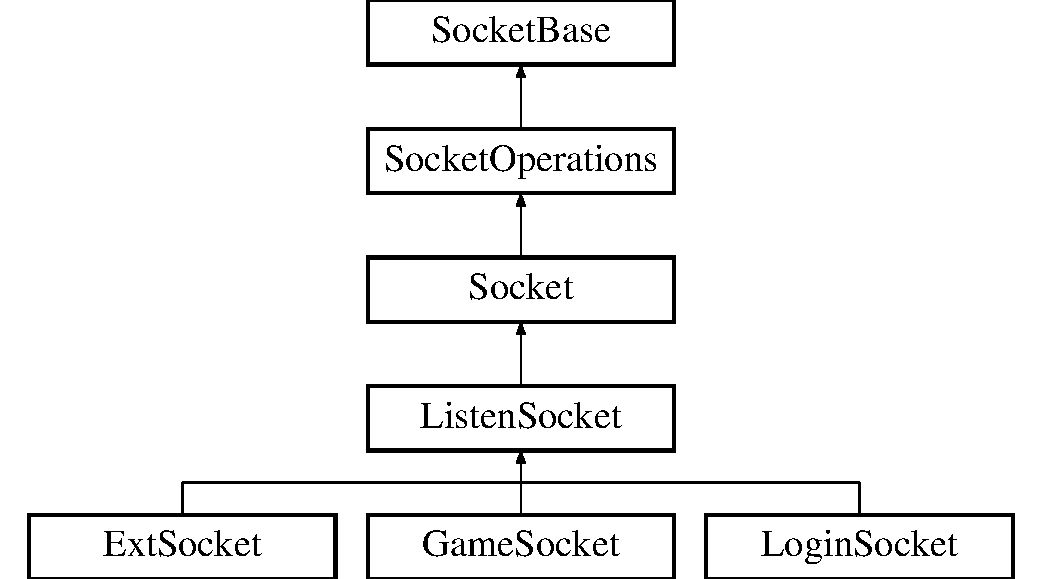
\includegraphics[height=5.000000cm]{classListenSocket}
\end{center}
\end{figure}
\subsection*{Public Member Functions}
\begin{DoxyCompactItemize}
\item 
\hypertarget{classListenSocket_a88bc05466de1c71e9981b1664a0631dd}{
{\bfseries ListenSocket} (const char $\ast$listen\_\-address, uint port)}
\label{classListenSocket_a88bc05466de1c71e9981b1664a0631dd}

\item 
\hypertarget{classListenSocket_ac62a573cd01cf0826e8d2a3872565e58}{
void {\bfseries onAccept} ()}
\label{classListenSocket_ac62a573cd01cf0826e8d2a3872565e58}

\item 
\hypertarget{classListenSocket_a611c169149189c64d3aa582806692350}{
void {\bfseries close} ()}
\label{classListenSocket_a611c169149189c64d3aa582806692350}

\end{DoxyCompactItemize}
\subsubsection*{template$<$class SocketClass$>$ class ListenSocket$<$ SocketClass $>$}



The documentation for this class was generated from the following file:\begin{DoxyCompactItemize}
\item 
/home/nonametr/projects/anima/shared/listensocket.h\end{DoxyCompactItemize}

\input{classlocation}
\input{classLoginSocket}
\input{classLoginSocketThread}
\input{classMainInstance}
\hypertarget{classMutex}{\section{\-Mutex \-Class \-Reference}
\label{classMutex}\index{\-Mutex@{\-Mutex}}
}
\subsection*{\-Public \-Member \-Functions}
\begin{DoxyCompactItemize}
\item 
\hyperlink{classMutex_a593423d868daf926c7b0d63a833ae29a}{\-Mutex} ()
\item 
virtual \hyperlink{classMutex_ac9e9182407f5f74892318607888e9be4}{$\sim$\-Mutex} ()
\item 
\hypertarget{classMutex_ad91be808bf0a60a16f10b897ec246d3a}{void {\bfseries lock} ()}\label{classMutex_ad91be808bf0a60a16f10b897ec246d3a}

\item 
\hypertarget{classMutex_a546a5b797ba29959357586aa2b3740a8}{void {\bfseries unlock} ()}\label{classMutex_a546a5b797ba29959357586aa2b3740a8}

\item 
bool \hyperlink{classMutex_a9dc89e7486c13d892d31a3795c8ea3cc}{try\-\_\-1k\-\_\-lock} ()
\item 
\hypertarget{classMutex_a85bdf2b7c3d9ce789c61f8bc2a127c8a}{bool {\bfseries try\-\_\-lock} ()}\label{classMutex_a85bdf2b7c3d9ce789c61f8bc2a127c8a}

\end{DoxyCompactItemize}
\subsection*{\-Protected \-Attributes}
\begin{DoxyCompactItemize}
\item 
pthread\-\_\-mutex\-\_\-t \hyperlink{classMutex_a8feb0b01916c1feedd1f0c0dcd74081b}{mutex}
\end{DoxyCompactItemize}
\subsection*{\-Static \-Protected \-Attributes}
\begin{DoxyCompactItemize}
\item 
\hypertarget{classMutex_ad7ee7f8bf85bcdc0cd99f7fb82cd9f83}{static bool {\bfseries attr\-\_\-initalized} = false}\label{classMutex_ad7ee7f8bf85bcdc0cd99f7fb82cd9f83}

\item 
\hypertarget{classMutex_a7c27b9401231941ebf4cce6cfc81192c}{static pthread\-\_\-mutexattr\-\_\-t {\bfseries attr}}\label{classMutex_a7c27b9401231941ebf4cce6cfc81192c}

\end{DoxyCompactItemize}


\subsection{\-Constructor \& \-Destructor \-Documentation}
\hypertarget{classMutex_a593423d868daf926c7b0d63a833ae29a}{\index{\-Mutex@{\-Mutex}!\-Mutex@{\-Mutex}}
\index{\-Mutex@{\-Mutex}!Mutex@{\-Mutex}}
\subsubsection[{\-Mutex}]{\setlength{\rightskip}{0pt plus 5cm}{\bf \-Mutex\-::\-Mutex} (
\begin{DoxyParamCaption}
{}
\end{DoxyParamCaption}
)}}\label{classMutex_a593423d868daf926c7b0d63a833ae29a}
\-Initializes a mutex class, with pthread\-\_\-mutex\-\_\-init \hypertarget{classMutex_ac9e9182407f5f74892318607888e9be4}{\index{\-Mutex@{\-Mutex}!$\sim$\-Mutex@{$\sim$\-Mutex}}
\index{$\sim$\-Mutex@{$\sim$\-Mutex}!Mutex@{\-Mutex}}
\subsubsection[{$\sim$\-Mutex}]{\setlength{\rightskip}{0pt plus 5cm}{\bf \-Mutex\-::$\sim$\-Mutex} (
\begin{DoxyParamCaption}
{}
\end{DoxyParamCaption}
)\hspace{0.3cm}{\ttfamily  \mbox{[}virtual\mbox{]}}}}\label{classMutex_ac9e9182407f5f74892318607888e9be4}
\-Deletes the associated mutex 

\subsection{\-Member \-Function \-Documentation}
\hypertarget{classMutex_a9dc89e7486c13d892d31a3795c8ea3cc}{\index{\-Mutex@{\-Mutex}!try\-\_\-1k\-\_\-lock@{try\-\_\-1k\-\_\-lock}}
\index{try\-\_\-1k\-\_\-lock@{try\-\_\-1k\-\_\-lock}!Mutex@{\-Mutex}}
\subsubsection[{try\-\_\-1k\-\_\-lock}]{\setlength{\rightskip}{0pt plus 5cm}bool {\bf \-Mutex\-::try\-\_\-1k\-\_\-lock} (
\begin{DoxyParamCaption}
{}
\end{DoxyParamCaption}
)\hspace{0.3cm}{\ttfamily  \mbox{[}inline\mbox{]}}}}\label{classMutex_a9dc89e7486c13d892d31a3795c8ea3cc}
\begin{DoxyReturn}{\-Returns}
false if cannot be lock, true if it was locked. 
\end{DoxyReturn}


\subsection{\-Member \-Data \-Documentation}
\hypertarget{classMutex_a8feb0b01916c1feedd1f0c0dcd74081b}{\index{\-Mutex@{\-Mutex}!mutex@{mutex}}
\index{mutex@{mutex}!Mutex@{\-Mutex}}
\subsubsection[{mutex}]{\setlength{\rightskip}{0pt plus 5cm}pthread\-\_\-mutex\-\_\-t {\bf \-Mutex\-::mutex}\hspace{0.3cm}{\ttfamily  \mbox{[}protected\mbox{]}}}}\label{classMutex_a8feb0b01916c1feedd1f0c0dcd74081b}
pthread struct used in system calls 

\-The documentation for this class was generated from the following files\-:\begin{DoxyCompactItemize}
\item 
/home/nonametr/projects/voodoo/server/shared/mt/thread.\-h\item 
/home/nonametr/projects/voodoo/server/shared/mt/thread.\-cpp\end{DoxyCompactItemize}

\input{classMySQLDatabase}
\input{structMySQLDatabaseConnection}
\input{classMySQLQueryResult}
\hypertarget{classNetCore}{\section{\-Net\-Core \-Class \-Reference}
\label{classNetCore}\index{\-Net\-Core@{\-Net\-Core}}
}
\-Inheritance diagram for \-Net\-Core\-:\begin{figure}[H]
\begin{center}
\leavevmode
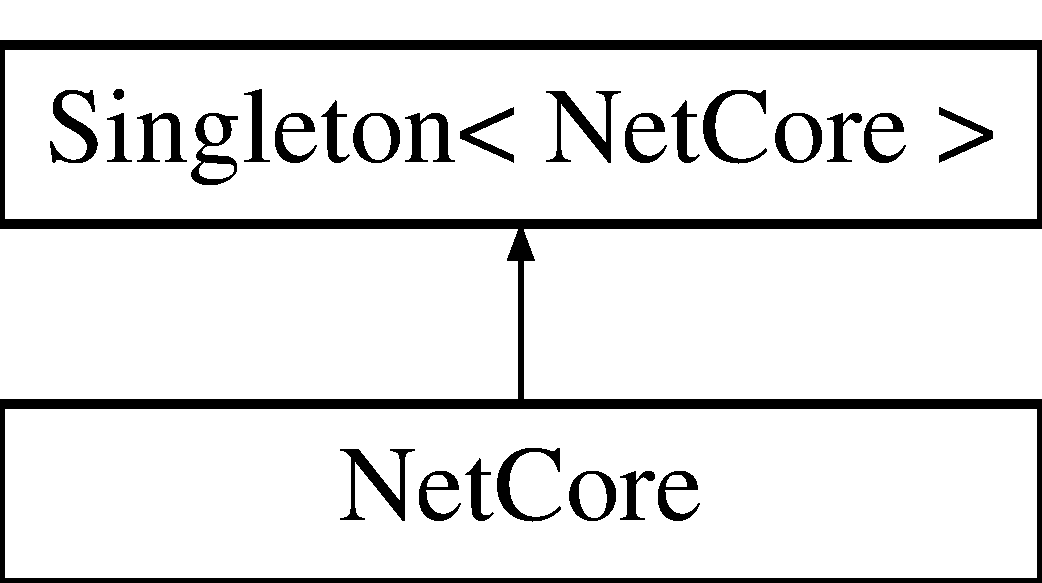
\includegraphics[height=2.000000cm]{classNetCore}
\end{center}
\end{figure}
\subsection*{\-Public \-Member \-Functions}
\begin{DoxyCompactItemize}
\item 
\hyperlink{classNetCore_ad10840be05aa99314c59ca10f067b2da}{\-Net\-Core} ()
\item 
void \hyperlink{classNetCore_a427f3577c790d9199e9e976172e32ea3}{add\-Socket} (\hyperlink{classSocket}{\-Socket} $\ast$s)
\begin{DoxyCompactList}\small\item\em add a new socket to the r/w epoll set and to the sock mapping \end{DoxyCompactList}\item 
\hypertarget{classNetCore_adae8b16fc82aed8f9b10ab4e431c886e}{void {\bfseries add\-Listen\-Socket} (\hyperlink{classListenSocket}{\-Listen\-Socket} $\ast$s)}\label{classNetCore_adae8b16fc82aed8f9b10ab4e431c886e}

\end{DoxyCompactItemize}
\subsection*{\-Friends}
\begin{DoxyCompactItemize}
\item 
\hypertarget{classNetCore_ae0585299ab7c2a563b1aeabf73ea2c21}{class {\bfseries \-Net\-Core\-Worker\-Thread}}\label{classNetCore_ae0585299ab7c2a563b1aeabf73ea2c21}

\item 
\hypertarget{classNetCore_ab510887d735ee73ab1cb598c66260e87}{class {\bfseries \-Socket}}\label{classNetCore_ab510887d735ee73ab1cb598c66260e87}

\end{DoxyCompactItemize}


\subsection{\-Constructor \& \-Destructor \-Documentation}
\hypertarget{classNetCore_ad10840be05aa99314c59ca10f067b2da}{\index{\-Net\-Core@{\-Net\-Core}!\-Net\-Core@{\-Net\-Core}}
\index{\-Net\-Core@{\-Net\-Core}!NetCore@{\-Net\-Core}}
\subsubsection[{\-Net\-Core}]{\setlength{\rightskip}{0pt plus 5cm}{\bf \-Net\-Core\-::\-Net\-Core} (
\begin{DoxyParamCaption}
{}
\end{DoxyParamCaption}
)}}\label{classNetCore_ad10840be05aa99314c59ca10f067b2da}
null out the pointer array 

\subsection{\-Member \-Function \-Documentation}
\hypertarget{classNetCore_a427f3577c790d9199e9e976172e32ea3}{\index{\-Net\-Core@{\-Net\-Core}!add\-Socket@{add\-Socket}}
\index{add\-Socket@{add\-Socket}!NetCore@{\-Net\-Core}}
\subsubsection[{add\-Socket}]{\setlength{\rightskip}{0pt plus 5cm}void {\bf \-Net\-Core\-::add\-Socket} (
\begin{DoxyParamCaption}
\item[{{\bf \-Socket} $\ast$}]{s}
\end{DoxyParamCaption}
)}}\label{classNetCore_a427f3577c790d9199e9e976172e32ea3}


add a new socket to the r/w epoll set and to the sock mapping 

clearing old sock obj. we clear it only if system returns same desc(system nows that its not in use long time ago \-:) 

\-The documentation for this class was generated from the following files\-:\begin{DoxyCompactItemize}
\item 
/home/nonametr/projects/voodoo/server/shared/net/net\-\_\-core.\-h\item 
/home/nonametr/projects/voodoo/server/shared/net/net\-\_\-core.\-cpp\end{DoxyCompactItemize}

\hypertarget{classNetCoreWorkerThread}{
\section{NetCoreWorkerThread Class Reference}
\label{classNetCoreWorkerThread}\index{NetCoreWorkerThread@{NetCoreWorkerThread}}
}
Inheritance diagram for NetCoreWorkerThread:\begin{figure}[H]
\begin{center}
\leavevmode
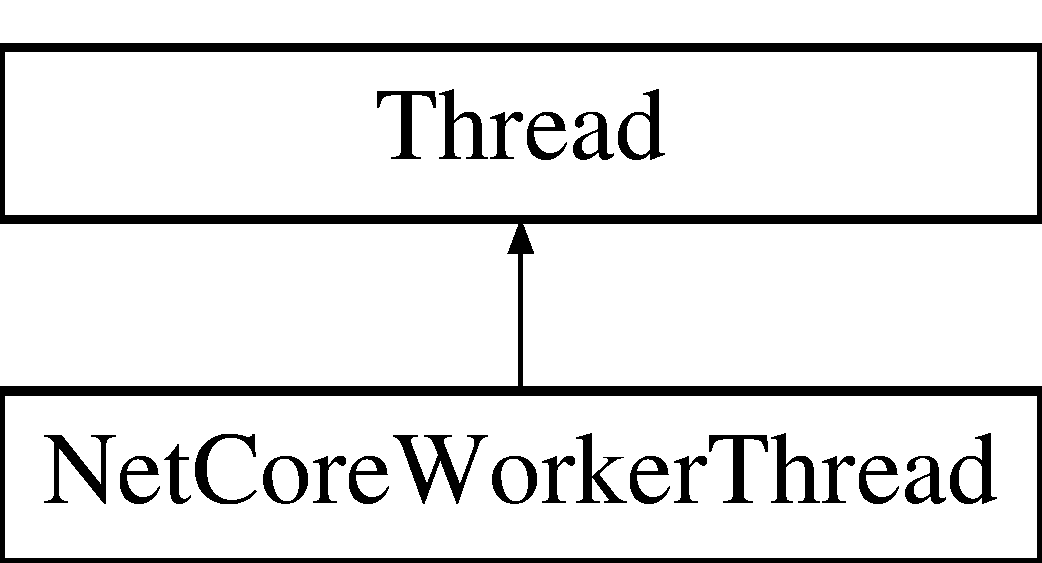
\includegraphics[height=2.000000cm]{classNetCoreWorkerThread}
\end{center}
\end{figure}
\subsection*{Public Member Functions}
\begin{DoxyCompactItemize}
\item 
\hypertarget{classNetCoreWorkerThread_a743b906293b9ed2c3bfc1749e6257187}{
void {\bfseries run} ()}
\label{classNetCoreWorkerThread_a743b906293b9ed2c3bfc1749e6257187}

\item 
\hypertarget{classNetCoreWorkerThread_a6ffdaca7b662d69cf305fbd8d9044222}{
void {\bfseries onShutdown} ()}
\label{classNetCoreWorkerThread_a6ffdaca7b662d69cf305fbd8d9044222}

\end{DoxyCompactItemize}
\subsection*{Friends}
\begin{DoxyCompactItemize}
\item 
\hypertarget{classNetCoreWorkerThread_ab3be64b93c69b019c9ecebf16700262d}{
class \hyperlink{classNetCoreWorkerThread_ab3be64b93c69b019c9ecebf16700262d}{NetCore}}
\label{classNetCoreWorkerThread_ab3be64b93c69b019c9ecebf16700262d}

\end{DoxyCompactItemize}


The documentation for this class was generated from the following files:\begin{DoxyCompactItemize}
\item 
/home/nonametr/projects/anima/shared/netcore.h\item 
/home/nonametr/projects/anima/shared/netcore.cpp\end{DoxyCompactItemize}

\input{classObject}
\input{classObjectList}
\input{structOG__ERROR}
\input{structOG__USER__JSON}
\hypertarget{structPacket}{
\section{Packet Struct Reference}
\label{structPacket}\index{Packet@{Packet}}
}
\subsection*{Public Attributes}
\begin{DoxyCompactItemize}
\item 
\hypertarget{structPacket_a98961f942ac0ff932175cd8558b93814}{
string {\bfseries data}}
\label{structPacket_a98961f942ac0ff932175cd8558b93814}

\item 
\hypertarget{structPacket_a182163515741c6f8310e9170dd994e8a}{
\hyperlink{classSocket}{Socket} $\ast$ {\bfseries connect}}
\label{structPacket_a182163515741c6f8310e9170dd994e8a}

\end{DoxyCompactItemize}


The documentation for this struct was generated from the following file:\begin{DoxyCompactItemize}
\item 
/home/nonametr/projects/anima/login\_\-server/loginserverhandler.h\end{DoxyCompactItemize}

\input{classPacketHandler}
\hypertarget{structPeriodicThread}{
\section{PeriodicThread Struct Reference}
\label{structPeriodicThread}\index{PeriodicThread@{PeriodicThread}}
}
\subsection*{Public Attributes}
\begin{DoxyCompactItemize}
\item 
\hypertarget{structPeriodicThread_acede129e7cdac21b9c693663ecd8cce8}{
std::vector$<$ \hyperlink{classThread}{Thread} $\ast$ $>$ {\bfseries threads\_\-to\_\-run}}
\label{structPeriodicThread_acede129e7cdac21b9c693663ecd8cce8}

\item 
\hypertarget{structPeriodicThread_a3abca614693acac7690c25795da551df}{
uint {\bfseries call\_\-interval}}
\label{structPeriodicThread_a3abca614693acac7690c25795da551df}

\end{DoxyCompactItemize}


The documentation for this struct was generated from the following file:\begin{DoxyCompactItemize}
\item 
/home/nonametr/projects/anima/shared/periodicthreadcaller.h\end{DoxyCompactItemize}

\hypertarget{classPeriodicThreadCaller}{\section{\-Periodic\-Thread\-Caller \-Class \-Reference}
\label{classPeriodicThreadCaller}\index{\-Periodic\-Thread\-Caller@{\-Periodic\-Thread\-Caller}}
}
\-Inheritance diagram for \-Periodic\-Thread\-Caller\-:\begin{figure}[H]
\begin{center}
\leavevmode
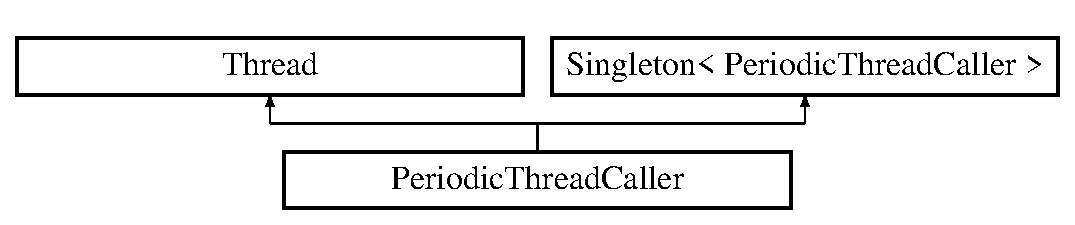
\includegraphics[height=2.000000cm]{classPeriodicThreadCaller}
\end{center}
\end{figure}
\subsection*{\-Public \-Member \-Functions}
\begin{DoxyCompactItemize}
\item 
virtual void \hyperlink{classPeriodicThreadCaller_ae57ca10be27bf07f027364b1fb507403}{run} ()
\item 
virtual void \hyperlink{classPeriodicThreadCaller_acef1ccc3857cabe56fd267fe986a13c7}{on\-Shutdown} ()
\item 
void \hyperlink{classPeriodicThreadCaller_af534285065e548ad5e0527620a39ea07}{start\-Periodic\-Thread} (\hyperlink{classThread}{\-Thread} $\ast$thread, uint32 call\-\_\-interval)
\end{DoxyCompactItemize}


\subsection{\-Member \-Function \-Documentation}
\hypertarget{classPeriodicThreadCaller_acef1ccc3857cabe56fd267fe986a13c7}{\index{\-Periodic\-Thread\-Caller@{\-Periodic\-Thread\-Caller}!on\-Shutdown@{on\-Shutdown}}
\index{on\-Shutdown@{on\-Shutdown}!PeriodicThreadCaller@{\-Periodic\-Thread\-Caller}}
\subsubsection[{on\-Shutdown}]{\setlength{\rightskip}{0pt plus 5cm}void {\bf \-Periodic\-Thread\-Caller\-::on\-Shutdown} (
\begin{DoxyParamCaption}
{}
\end{DoxyParamCaption}
)\hspace{0.3cm}{\ttfamily  \mbox{[}virtual\mbox{]}}}}\label{classPeriodicThreadCaller_acef1ccc3857cabe56fd267fe986a13c7}
waiking up periodic thread callback checks 

\-Implements \hyperlink{classThread}{\-Thread}.

\hypertarget{classPeriodicThreadCaller_ae57ca10be27bf07f027364b1fb507403}{\index{\-Periodic\-Thread\-Caller@{\-Periodic\-Thread\-Caller}!run@{run}}
\index{run@{run}!PeriodicThreadCaller@{\-Periodic\-Thread\-Caller}}
\subsubsection[{run}]{\setlength{\rightskip}{0pt plus 5cm}void {\bf \-Periodic\-Thread\-Caller\-::run} (
\begin{DoxyParamCaption}
{}
\end{DoxyParamCaption}
)\hspace{0.3cm}{\ttfamily  \mbox{[}virtual\mbox{]}}}}\label{classPeriodicThreadCaller_ae57ca10be27bf07f027364b1fb507403}
its next exam\-\_\-time 

\-Implements \hyperlink{classThread}{\-Thread}.

\hypertarget{classPeriodicThreadCaller_af534285065e548ad5e0527620a39ea07}{\index{\-Periodic\-Thread\-Caller@{\-Periodic\-Thread\-Caller}!start\-Periodic\-Thread@{start\-Periodic\-Thread}}
\index{start\-Periodic\-Thread@{start\-Periodic\-Thread}!PeriodicThreadCaller@{\-Periodic\-Thread\-Caller}}
\subsubsection[{start\-Periodic\-Thread}]{\setlength{\rightskip}{0pt plus 5cm}void {\bf \-Periodic\-Thread\-Caller\-::start\-Periodic\-Thread} (
\begin{DoxyParamCaption}
\item[{{\bf \-Thread} $\ast$}]{thread, }
\item[{uint32}]{call\-\_\-interval}
\end{DoxyParamCaption}
)}}\label{classPeriodicThreadCaller_af534285065e548ad5e0527620a39ea07}
waiking up periodic thread callback checks 

\-The documentation for this class was generated from the following files\-:\begin{DoxyCompactItemize}
\item 
/home/nonametr/projects/voodoo/server/shared/mt/periodic\-\_\-thread\-\_\-caller.\-h\item 
/home/nonametr/projects/voodoo/server/shared/mt/periodic\-\_\-thread\-\_\-caller.\-cpp\end{DoxyCompactItemize}

\input{classQueryBuffer}
\input{classQueryResult}
\input{classQueryThread}
\input{classRandom}
\input{classRatingManager}
\input{classReferenceCounter}
\input{classServer}
\hypertarget{classSingleton}{\section{\-Singleton$<$ type $>$ \-Class \-Template \-Reference}
\label{classSingleton}\index{\-Singleton$<$ type $>$@{\-Singleton$<$ type $>$}}
}
\subsection*{\-Public \-Member \-Functions}
\begin{DoxyCompactItemize}
\item 
\hypertarget{classSingleton_ae4796cfb8f04fba7bb556e2a8c389162}{virtual \hyperlink{classSingleton_ae4796cfb8f04fba7bb556e2a8c389162}{$\sim$\-Singleton} ()}\label{classSingleton_ae4796cfb8f04fba7bb556e2a8c389162}

\begin{DoxyCompactList}\small\item\em \-Destructor. \end{DoxyCompactList}\end{DoxyCompactItemize}
\subsection*{\-Static \-Public \-Member \-Functions}
\begin{DoxyCompactItemize}
\item 
\hypertarget{classSingleton_a5c8fb723215374aecde038fe7ca205fc}{static type \& {\bfseries get\-Singleton} ()}\label{classSingleton_a5c8fb723215374aecde038fe7ca205fc}

\item 
\hypertarget{classSingleton_a86b173e3d50f8a902380f354f2213677}{static type $\ast$ {\bfseries get\-Singleton\-Ptr} ()}\label{classSingleton_a86b173e3d50f8a902380f354f2213677}

\end{DoxyCompactItemize}
\subsection*{\-Protected \-Member \-Functions}
\begin{DoxyCompactItemize}
\item 
\hyperlink{classSingleton_ab357f8b89622a5207c7c3e58bf43bfb9}{\-Singleton} ()
\begin{DoxyCompactList}\small\item\em \-Constructor. \end{DoxyCompactList}\end{DoxyCompactItemize}
\subsubsection*{template$<$class type$>$ class Singleton$<$ type $>$}



\subsection{\-Constructor \& \-Destructor \-Documentation}
\hypertarget{classSingleton_ab357f8b89622a5207c7c3e58bf43bfb9}{\index{\-Singleton@{\-Singleton}!\-Singleton@{\-Singleton}}
\index{\-Singleton@{\-Singleton}!Singleton@{\-Singleton}}
\subsubsection[{\-Singleton}]{\setlength{\rightskip}{0pt plus 5cm}template$<$class type$>$ {\bf \-Singleton}$<$ type $>$\-::{\bf \-Singleton} (
\begin{DoxyParamCaption}
{}
\end{DoxyParamCaption}
)\hspace{0.3cm}{\ttfamily  \mbox{[}inline, protected\mbox{]}}}}\label{classSingleton_ab357f8b89622a5207c7c3e58bf43bfb9}


\-Constructor. 

\-If you hit this assert, this singleton already exists -\/-\/ you can't create another one! 

\-The documentation for this class was generated from the following file\-:\begin{DoxyCompactItemize}
\item 
/home/nonametr/projects/voodoo/server/shared/singleton.\-h\end{DoxyCompactItemize}

\input{classSmartPtr}
\input{structSocialNetDesc}
\hypertarget{classSocket}{\section{\-Socket \-Class \-Reference}
\label{classSocket}\index{\-Socket@{\-Socket}}
}
\-Inheritance diagram for \-Socket\-:\begin{figure}[H]
\begin{center}
\leavevmode
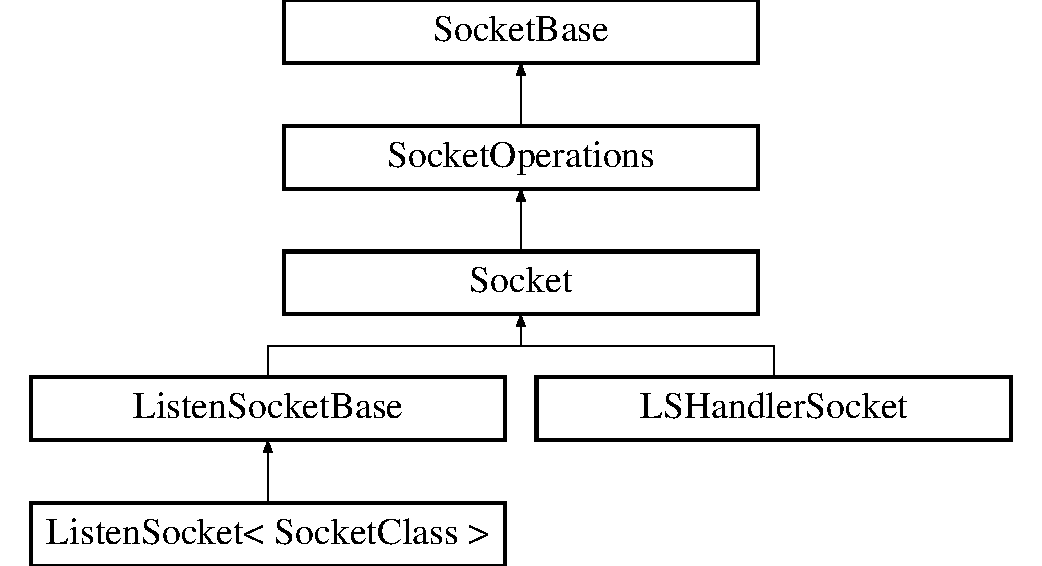
\includegraphics[height=5.000000cm]{classSocket}
\end{center}
\end{figure}
\subsection*{\-Public \-Types}
\begin{DoxyCompactItemize}
\item 
enum {\bfseries \-Sock\-Type} \{ {\bfseries \-D\-E\-F\-A\-U\-L\-T\-\_\-\-S\-O\-C\-K\-E\-T} =  0, 
{\bfseries \-H\-T\-T\-P\-\_\-\-S\-O\-C\-K\-E\-T}
 \}
\end{DoxyCompactItemize}
\subsection*{\-Public \-Member \-Functions}
\begin{DoxyCompactItemize}
\item 
\hypertarget{classSocket_acba9bcb13219372b3236ebd45edc29fb}{{\bfseries \-Socket} (int sock)}\label{classSocket_acba9bcb13219372b3236ebd45edc29fb}

\item 
\hypertarget{classSocket_a05d03ffaefb03f6bb07e5f5dcdb8c3cd}{void \hyperlink{classSocket_a05d03ffaefb03f6bb07e5f5dcdb8c3cd}{connect} (const char $\ast$address, uint32 port)}\label{classSocket_a05d03ffaefb03f6bb07e5f5dcdb8c3cd}

\begin{DoxyCompactList}\small\item\em \-Open a connection to another machine. \end{DoxyCompactList}\item 
\hypertarget{classSocket_a0aed22a4e59d0492ee5ed6d5c89ef762}{void \hyperlink{classSocket_a0aed22a4e59d0492ee5ed6d5c89ef762}{disconnect} ()}\label{classSocket_a0aed22a4e59d0492ee5ed6d5c89ef762}

\begin{DoxyCompactList}\small\item\em \-Disconnect the socket. \end{DoxyCompactList}\item 
\hypertarget{classSocket_a2d86a782f8bd8c002a4a92feffaf0180}{void \hyperlink{classSocket_a2d86a782f8bd8c002a4a92feffaf0180}{accept} (sockaddr\-\_\-in $\ast$address)}\label{classSocket_a2d86a782f8bd8c002a4a92feffaf0180}

\begin{DoxyCompactList}\small\item\em \-Accept from connection. \end{DoxyCompactList}\item 
\hypertarget{classSocket_abe848a0d3a96711d1cc0a8c10d5d066b}{void \hyperlink{classSocket_abe848a0d3a96711d1cc0a8c10d5d066b}{send} (const char $\ast$out\-\_\-packet, uint32 size)}\label{classSocket_abe848a0d3a96711d1cc0a8c10d5d066b}

\begin{DoxyCompactList}\small\item\em \-Send bytes. \end{DoxyCompactList}\item 
\hypertarget{classSocket_ae77c62ce4c867e1ae501fbc355bf9f6a}{void {\bfseries send} (\hyperlink{structPacket}{\-Packet} $\ast$pkt)}\label{classSocket_ae77c62ce4c867e1ae501fbc355bf9f6a}

\item 
\hypertarget{classSocket_a89fd9c15aa0807c03543d9ba79b2c4a7}{void \hyperlink{classSocket_a89fd9c15aa0807c03543d9ba79b2c4a7}{read} ()}\label{classSocket_a89fd9c15aa0807c03543d9ba79b2c4a7}

\begin{DoxyCompactList}\small\item\em \-Read bytes. \end{DoxyCompactList}\item 
\hypertarget{classSocket_a80de761d2722d0aea1b2b16867b30996}{void {\bfseries set\-Owner} (\hyperlink{classListenSocket}{\-Listen\-Socket} $\ast$owner)}\label{classSocket_a80de761d2722d0aea1b2b16867b30996}

\item 
\hypertarget{classSocket_a60c76a4c1e26192218d598b63cbb97b9}{bool {\bfseries is\-Connected} ()}\label{classSocket_a60c76a4c1e26192218d598b63cbb97b9}

\item 
\hypertarget{classSocket_ab54ab05b7088f40f9b9c9704d313cc68}{string {\bfseries get\-Remote\-I\-P} ()}\label{classSocket_ab54ab05b7088f40f9b9c9704d313cc68}

\item 
\hypertarget{classSocket_a00b515650b6ac528d997e1afe7787197}{uint32 {\bfseries get\-Remote\-Port} ()}\label{classSocket_a00b515650b6ac528d997e1afe7787197}

\item 
\hypertarget{classSocket_a7d9eae997fba47664fdc87227f3ed2e8}{in\-\_\-addr {\bfseries get\-Remote\-Address} ()}\label{classSocket_a7d9eae997fba47664fdc87227f3ed2e8}

\item 
\hypertarget{classSocket_aa0e1cac0aa5ca19e32e035bb2dce77a4}{void {\bfseries set\-Type} (\-Sock\-Type v\-\_\-type)}\label{classSocket_aa0e1cac0aa5ca19e32e035bb2dce77a4}

\item 
\hypertarget{classSocket_ae003b7c284944cfa8fe7662ebd82b666}{\-Sock\-Type {\bfseries get\-Type} ()}\label{classSocket_ae003b7c284944cfa8fe7662ebd82b666}

\end{DoxyCompactItemize}


\-The documentation for this class was generated from the following files\-:\begin{DoxyCompactItemize}
\item 
/home/nonametr/projects/voodoo/server/shared/net/socket.\-h\item 
/home/nonametr/projects/voodoo/server/shared/net/socket.\-cpp\end{DoxyCompactItemize}

\hypertarget{classSocketBase}{\section{\-Socket\-Base \-Class \-Reference}
\label{classSocketBase}\index{\-Socket\-Base@{\-Socket\-Base}}
}
\-Inheritance diagram for \-Socket\-Base\-:\begin{figure}[H]
\begin{center}
\leavevmode
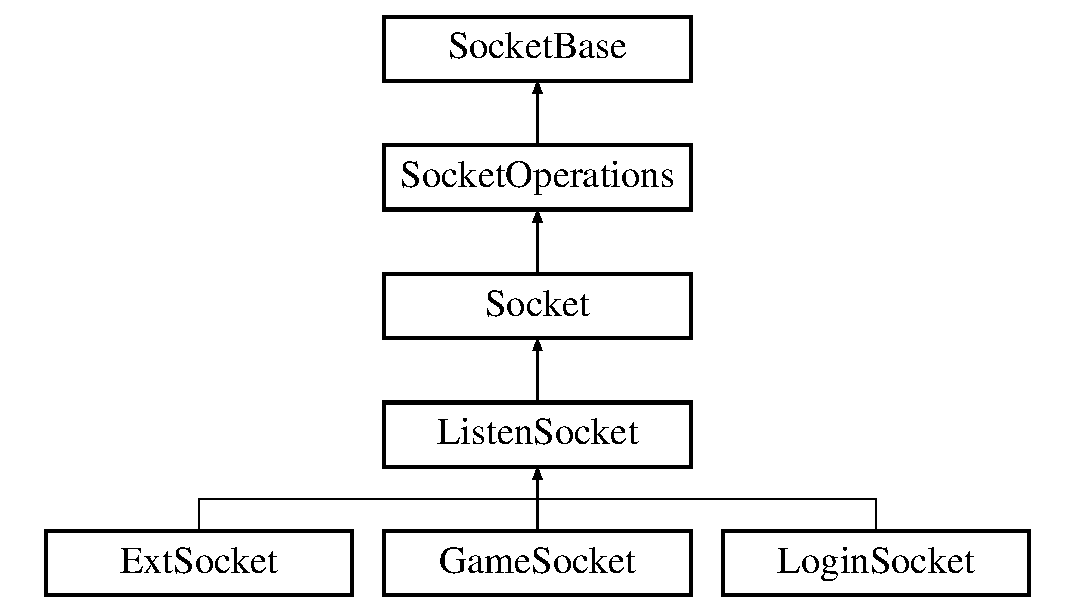
\includegraphics[height=5.000000cm]{classSocketBase}
\end{center}
\end{figure}
\subsection*{\-Public \-Member \-Functions}
\begin{DoxyCompactItemize}
\item 
\hypertarget{classSocketBase_ab32e06f32c8762d4261b98793fabcf06}{\-S\-O\-C\-K\-E\-T {\bfseries get\-Sock\-Descriptor} ()}\label{classSocketBase_ab32e06f32c8762d4261b98793fabcf06}

\end{DoxyCompactItemize}
\subsection*{\-Protected \-Attributes}
\begin{DoxyCompactItemize}
\item 
\hypertarget{classSocketBase_a07179135c511d69e46cb29fcb1c2b8af}{\-S\-O\-C\-K\-E\-T {\bfseries \-\_\-sock}}\label{classSocketBase_a07179135c511d69e46cb29fcb1c2b8af}

\end{DoxyCompactItemize}


\-The documentation for this class was generated from the following file\-:\begin{DoxyCompactItemize}
\item 
/home/nonametr/projects/voodoo/server/shared/net/socket\-\_\-base.\-h\end{DoxyCompactItemize}

\hypertarget{classSocketOperations}{\section{\-Socket\-Operations \-Class \-Reference}
\label{classSocketOperations}\index{\-Socket\-Operations@{\-Socket\-Operations}}
}
\-Inheritance diagram for \-Socket\-Operations\-:\begin{figure}[H]
\begin{center}
\leavevmode
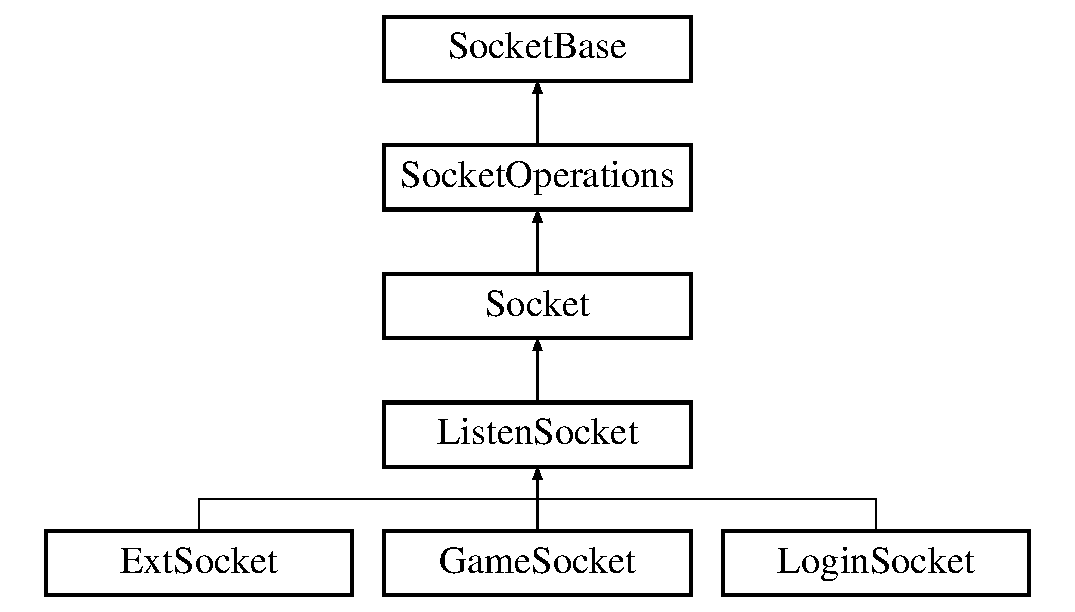
\includegraphics[height=5.000000cm]{classSocketOperations}
\end{center}
\end{figure}
\subsection*{\-Public \-Member \-Functions}
\begin{DoxyCompactItemize}
\item 
\-S\-O\-C\-K\-E\-T \hyperlink{classSocketOperations_a542d416133a25018961be5703cc82d8f}{create} ()
\begin{DoxyCompactList}\small\item\em \-Create file descriptor for socket i/o operations. \end{DoxyCompactList}\item 
\hypertarget{classSocketOperations_a342adc61aee2904e6b6b2b650ee30c64}{bool \hyperlink{classSocketOperations_a342adc61aee2904e6b6b2b650ee30c64}{disable\-Blocking} ()}\label{classSocketOperations_a342adc61aee2904e6b6b2b650ee30c64}

\begin{DoxyCompactList}\small\item\em \-Disable blocking send/recv calls. \end{DoxyCompactList}\item 
\hypertarget{classSocketOperations_afa7bbc20f36191bb502975072f1c1bcf}{bool \hyperlink{classSocketOperations_afa7bbc20f36191bb502975072f1c1bcf}{disable\-Buffering} ()}\label{classSocketOperations_afa7bbc20f36191bb502975072f1c1bcf}

\begin{DoxyCompactList}\small\item\em \-Disable nagle buffering algorithm. \end{DoxyCompactList}\item 
\hypertarget{classSocketOperations_a136fe3ab807a04ae165f90f034d27628}{bool \hyperlink{classSocketOperations_a136fe3ab807a04ae165f90f034d27628}{enable\-Buffering} ()}\label{classSocketOperations_a136fe3ab807a04ae165f90f034d27628}

\begin{DoxyCompactList}\small\item\em \-Enable nagle buffering algorithm. \end{DoxyCompactList}\item 
\hypertarget{classSocketOperations_a5ad20ec31c2576776c1ff2d1a69a6bda}{bool \hyperlink{classSocketOperations_a5ad20ec31c2576776c1ff2d1a69a6bda}{set\-Send\-Buffer\-Size} (uint32 size)}\label{classSocketOperations_a5ad20ec31c2576776c1ff2d1a69a6bda}

\begin{DoxyCompactList}\small\item\em \-Set internal buffer size to socket. \end{DoxyCompactList}\item 
\hypertarget{classSocketOperations_a1211a4834c1a9cc56023d6ac503be8e2}{bool \hyperlink{classSocketOperations_a1211a4834c1a9cc56023d6ac503be8e2}{set\-Recv\-Buffer\-Size} (uint32 size)}\label{classSocketOperations_a1211a4834c1a9cc56023d6ac503be8e2}

\begin{DoxyCompactList}\small\item\em \-Set internal buffer size to socket. \end{DoxyCompactList}\item 
\hypertarget{classSocketOperations_abb3710e2f6782f3d9853ee1e2bd6283d}{bool \hyperlink{classSocketOperations_abb3710e2f6782f3d9853ee1e2bd6283d}{set\-Timeout} (uint32 timeout)}\label{classSocketOperations_abb3710e2f6782f3d9853ee1e2bd6283d}

\begin{DoxyCompactList}\small\item\em \-Set internal timeout. \end{DoxyCompactList}\item 
\hypertarget{classSocketOperations_a9ab40fe87bfbcbe324b2138be424f00f}{bool \hyperlink{classSocketOperations_a9ab40fe87bfbcbe324b2138be424f00f}{set\-Keep\-Alive} ()}\label{classSocketOperations_a9ab40fe87bfbcbe324b2138be424f00f}

\begin{DoxyCompactList}\small\item\em \-Set socket keep alive. \end{DoxyCompactList}\item 
\hypertarget{classSocketOperations_aab33b81b1521f6bb1085b893b3d5ae52}{void \hyperlink{classSocketOperations_aab33b81b1521f6bb1085b893b3d5ae52}{close\-Socket} ()}\label{classSocketOperations_aab33b81b1521f6bb1085b893b3d5ae52}

\begin{DoxyCompactList}\small\item\em \-Closes a socket fully. \end{DoxyCompactList}\item 
\hypertarget{classSocketOperations_a1f5834a875fd7588196a412402b7ac2b}{void \hyperlink{classSocketOperations_a1f5834a875fd7588196a412402b7ac2b}{reuse\-Addr} ()}\label{classSocketOperations_a1f5834a875fd7588196a412402b7ac2b}

\begin{DoxyCompactList}\small\item\em \-Sets reuseaddr. \end{DoxyCompactList}\end{DoxyCompactItemize}


\subsection{\-Member \-Function \-Documentation}
\hypertarget{classSocketOperations_a542d416133a25018961be5703cc82d8f}{\index{\-Socket\-Operations@{\-Socket\-Operations}!create@{create}}
\index{create@{create}!SocketOperations@{\-Socket\-Operations}}
\subsubsection[{create}]{\setlength{\rightskip}{0pt plus 5cm}\-S\-O\-C\-K\-E\-T {\bf \-Socket\-Operations\-::create} (
\begin{DoxyParamCaption}
{}
\end{DoxyParamCaption}
)\hspace{0.3cm}{\ttfamily  \mbox{[}inline\mbox{]}}}}\label{classSocketOperations_a542d416133a25018961be5703cc82d8f}


\-Create file descriptor for socket i/o operations. 

create a socket for use with overlapped i/o 

\-The documentation for this class was generated from the following file\-:\begin{DoxyCompactItemize}
\item 
/home/nonametr/projects/voodoo/server/shared/net/socket\-\_\-operations.\-h\end{DoxyCompactItemize}

\input{classSQLCallbackBase}
\input{classSQLClassCallbackP0}
\input{classSQLClassCallbackP1}
\input{classSQLClassCallbackP2}
\input{classSQLClassCallbackP3}
\input{classSQLClassCallbackP4}
\input{classSQLFunctionCallbackP0}
\input{classSQLFunctionCallbackP1}
\input{classStorage}
\input{classStorageThread}
\input{classStorageTimer}
\hypertarget{classThread}{\section{\-Thread \-Class \-Reference}
\label{classThread}\index{\-Thread@{\-Thread}}
}
\-Inheritance diagram for \-Thread\-:\begin{figure}[H]
\begin{center}
\leavevmode
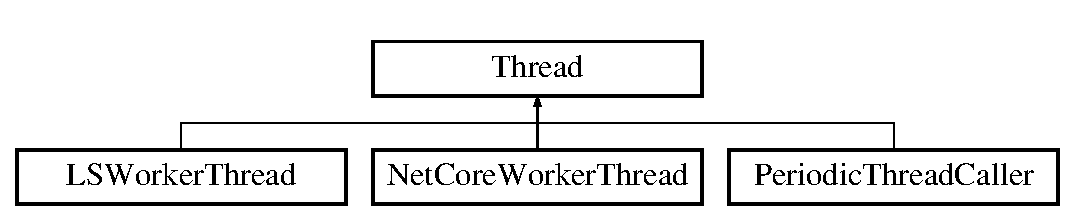
\includegraphics[height=11.000000cm]{classThread}
\end{center}
\end{figure}
\subsection*{\-Public \-Member \-Functions}
\begin{DoxyCompactItemize}
\item 
\hypertarget{classThread_aae90dfabab3e1776cf01a26e7ee3a620}{virtual void {\bfseries run} ()=0}\label{classThread_aae90dfabab3e1776cf01a26e7ee3a620}

\item 
\hypertarget{classThread_a9e30c8ade61860ebed96ce7ae5d0c0c1}{virtual void {\bfseries on\-Shutdown} ()=0}\label{classThread_a9e30c8ade61860ebed96ce7ae5d0c0c1}

\item 
\hypertarget{classThread_a39d788a3763b73e731196443edd4861f}{uint32 \hyperlink{classThread_a39d788a3763b73e731196443edd4861f}{get\-Tid} ()}\label{classThread_a39d788a3763b73e731196443edd4861f}

\begin{DoxyCompactList}\small\item\em it should be almost atomic. no general mutex locks \end{DoxyCompactList}\item 
\hypertarget{classThread_aec61ef8c40be81a63837315bc659c1a9}{void {\bfseries set\-Tid} (uint32 tid)}\label{classThread_aec61ef8c40be81a63837315bc659c1a9}

\end{DoxyCompactItemize}


\-The documentation for this class was generated from the following file\-:\begin{DoxyCompactItemize}
\item 
/home/nonametr/projects/voodoo/server/shared/mt/thread.\-h\end{DoxyCompactItemize}

\hypertarget{classThreadController}{
\section{ThreadController Class Reference}
\label{classThreadController}\index{ThreadController@{ThreadController}}
}
\subsection*{Public Member Functions}
\begin{DoxyCompactItemize}
\item 
\hypertarget{classThreadController_a7f95421885845c035d977fe0340784af}{
{\bfseries ThreadController} (uint thread\_\-id)}
\label{classThreadController_a7f95421885845c035d977fe0340784af}

\item 
\hypertarget{classThreadController_abcb1eeeade9465f8b9d288ce05a35b90}{
void {\bfseries setDeleteOnExit} (bool delete\_\-on\_\-exit)}
\label{classThreadController_abcb1eeeade9465f8b9d288ce05a35b90}

\item 
\hypertarget{classThreadController_a9cd2328f7af385c70a37a5f07d449bdb}{
void {\bfseries setup} (pthread\_\-t h)}
\label{classThreadController_a9cd2328f7af385c70a37a5f07d449bdb}

\item 
\hypertarget{classThreadController_a0c1ccf8af0171905931023efbf45ea5c}{
void {\bfseries setExecutionTarget} (\hyperlink{classThread}{Thread} $\ast$target)}
\label{classThreadController_a0c1ccf8af0171905931023efbf45ea5c}

\item 
\hypertarget{classThreadController_a78662807f4c0bf1714f2aeefe6205ced}{
void {\bfseries suspend} ()}
\label{classThreadController_a78662807f4c0bf1714f2aeefe6205ced}

\item 
\hypertarget{classThreadController_a53489422689e5ddcffde97d5c726154a}{
void {\bfseries resume} ()}
\label{classThreadController_a53489422689e5ddcffde97d5c726154a}

\item 
\hypertarget{classThreadController_a74a5e83564dcde1144f6c2d9394bd6ab}{
void {\bfseries run} ()}
\label{classThreadController_a74a5e83564dcde1144f6c2d9394bd6ab}

\item 
\hypertarget{classThreadController_ad150063920776421824399b975996117}{
void {\bfseries stop} ()}
\label{classThreadController_ad150063920776421824399b975996117}

\item 
\hypertarget{classThreadController_a3825c8c75845c86c48ea1f4caabfc3f5}{
void {\bfseries onShutdown} ()}
\label{classThreadController_a3825c8c75845c86c48ea1f4caabfc3f5}

\item 
\hypertarget{classThreadController_a945a302b689835971081b21a57c16023}{
\hyperlink{classThread}{Thread} $\ast$ {\bfseries getTarget} ()}
\label{classThreadController_a945a302b689835971081b21a57c16023}

\item 
\hypertarget{classThreadController_a6cc4c389d03bb41a87f495dc01291c03}{
bool {\bfseries isRuning} ()}
\label{classThreadController_a6cc4c389d03bb41a87f495dc01291c03}

\item 
\hypertarget{classThreadController_a2dd979e4429cff919c2fd12fa02c1394}{
void {\bfseries join} ()}
\label{classThreadController_a2dd979e4429cff919c2fd12fa02c1394}

\item 
\hypertarget{classThreadController_a9b29bed97f0135ffef8bbffe11221f38}{
uint {\bfseries getId} ()}
\label{classThreadController_a9b29bed97f0135ffef8bbffe11221f38}

\end{DoxyCompactItemize}


The documentation for this class was generated from the following file:\begin{DoxyCompactItemize}
\item 
/home/nonametr/projects/anima/shared/thread\_\-controller.h\end{DoxyCompactItemize}

\hypertarget{classThreadCore}{
\section{ThreadCore Class Reference}
\label{classThreadCore}\index{ThreadCore@{ThreadCore}}
}
Inheritance diagram for ThreadCore:\begin{figure}[H]
\begin{center}
\leavevmode
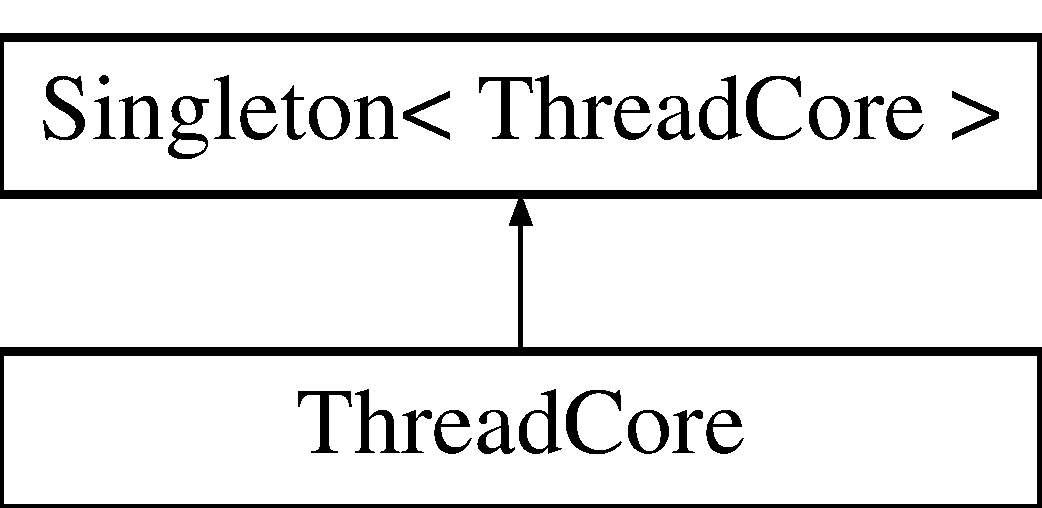
\includegraphics[height=2.000000cm]{classThreadCore}
\end{center}
\end{figure}
\subsection*{Public Member Functions}
\begin{DoxyCompactItemize}
\item 
\hyperlink{classThreadController}{ThreadController} $\ast$ \hyperlink{classThreadCore_acbbb91b15ac93fd819f0902383c212f8}{startThread} (\hyperlink{classThread}{Thread} $\ast$thread)
\begin{DoxyCompactList}\small\item\em tries to use precreated thread, if not found free one than creates a new thread \item\end{DoxyCompactList}\item 
\hypertarget{classThreadCore_a9ca50195858c2eb8b86e5fa00a7aba1a}{
void {\bfseries startThreadNoDel} (\hyperlink{classThread}{Thread} $\ast$thread)}
\label{classThreadCore_a9ca50195858c2eb8b86e5fa00a7aba1a}

\item 
bool \hyperlink{classThreadCore_a5dbcca9aafed540a2a07575e0ebe19a2}{threadExit} (\hyperlink{classThreadController}{ThreadController} $\ast$t\_\-control)
\item 
void \hyperlink{classThreadCore_a2144d2258b27e93b395b6108a52f03e0}{shutdown} ()
\end{DoxyCompactItemize}


\subsection{Member Function Documentation}
\hypertarget{classThreadCore_a2144d2258b27e93b395b6108a52f03e0}{
\index{ThreadCore@{ThreadCore}!shutdown@{shutdown}}
\index{shutdown@{shutdown}!ThreadCore@{ThreadCore}}
\subsubsection[{shutdown}]{\setlength{\rightskip}{0pt plus 5cm}void ThreadCore::shutdown (
\begin{DoxyParamCaption}
{}
\end{DoxyParamCaption}
)}}
\label{classThreadCore_a2144d2258b27e93b395b6108a52f03e0}


if we are here then a thread in the free pool checked if it was being shut down just before \hyperlink{classThreadCore_a2144d2258b27e93b395b6108a52f03e0}{shutdown()} was called, but called suspend() just after killing free threads. All we need to do is to resume it. 

\hypertarget{classThreadCore_acbbb91b15ac93fd819f0902383c212f8}{
\index{ThreadCore@{ThreadCore}!startThread@{startThread}}
\index{startThread@{startThread}!ThreadCore@{ThreadCore}}
\subsubsection[{startThread}]{\setlength{\rightskip}{0pt plus 5cm}{\bf ThreadController} $\ast$ ThreadCore::startThread (
\begin{DoxyParamCaption}
\item[{{\bf Thread} $\ast$}]{thread}
\end{DoxyParamCaption}
)}}
\label{classThreadCore_acbbb91b15ac93fd819f0902383c212f8}


tries to use precreated thread, if not found free one than creates a new thread 



grab one from the pool, if we have any

execute the task on this thread

resume the thread, and it should start working

creating a aditional new thread 

\hypertarget{classThreadCore_a5dbcca9aafed540a2a07575e0ebe19a2}{
\index{ThreadCore@{ThreadCore}!threadExit@{threadExit}}
\index{threadExit@{threadExit}!ThreadCore@{ThreadCore}}
\subsubsection[{threadExit}]{\setlength{\rightskip}{0pt plus 5cm}bool ThreadCore::threadExit (
\begin{DoxyParamCaption}
\item[{{\bf ThreadController} $\ast$}]{t\_\-control}
\end{DoxyParamCaption}
)}}
\label{classThreadCore_a5dbcca9aafed540a2a07575e0ebe19a2}


we're definitely no longer active

enter the \char`\"{}suspended\char`\"{} pool 



The documentation for this class was generated from the following files:\begin{DoxyCompactItemize}
\item 
/home/nonametr/projects/anima/shared/threadcore.h\item 
/home/nonametr/projects/anima/shared/threadcore.cpp\end{DoxyCompactItemize}

\input{classUser}
\input{classUserExt}
\input{classUserInterface}
\input{classValue}
\input{classVCBase}
\input{classVersionControl}
\printindex
\end{document}
